\chapter{Deep Learning Introduction into Knowledge-Based Systems}
\label{chap:dlintegrationkbs} 

This chapter \blfootnote{Amador-Domínguez, E., Serrano, E., Manrique, D., & Bajo, J. (2021). A Case-Based Reasoning Model Powered by Deep Learning for Radiology Report Recommendation. Int. J. Interact. Multim. Artif. Intell., 7(2), 15. doi:10.9781/ijimai.2021.08.011}presents the second insertion integration between deep learning models and knowledge-based systems. Section \ref{5_sec:dl_intro_kbs_methodology} presents the method parameters for the insertion of deep learning models in a knowledge-based system. This insertion method is instantiated into a hybrid framework, combining a case-based reasoning (CBR) model with different deep learning modules. Section \ref{5_sec:dl_powered_kbs_medical} outlines the main features of the proposed framework, focusing on its application in the medical domain. In this context, a CBR powered by DL modules for the generation of medical reports is presented. This scenario showcases the benefits of the introduction of DL into a CBR model, such as enabling reasoning over complex data (i.e., textual reports and images) or enhanced scalability. Section \ref{5_sec:raidologist} instantiates the proposed framework in its use for radiological report generation. Section \ref{5_sec:experimental_results} presents the experimental results. The compliance of the case scenario regarding the general design method is outlined in Section \ref{5_sec:design_compliance}. The chapter is summarized in Section \ref{5_sec:summary}. 


\section{Deep Learning Insertion in Knowledge-Based Systems}\label{5_sec:dl_intro_kbs_methodology}
\begin{figure}[t]
    \centering
    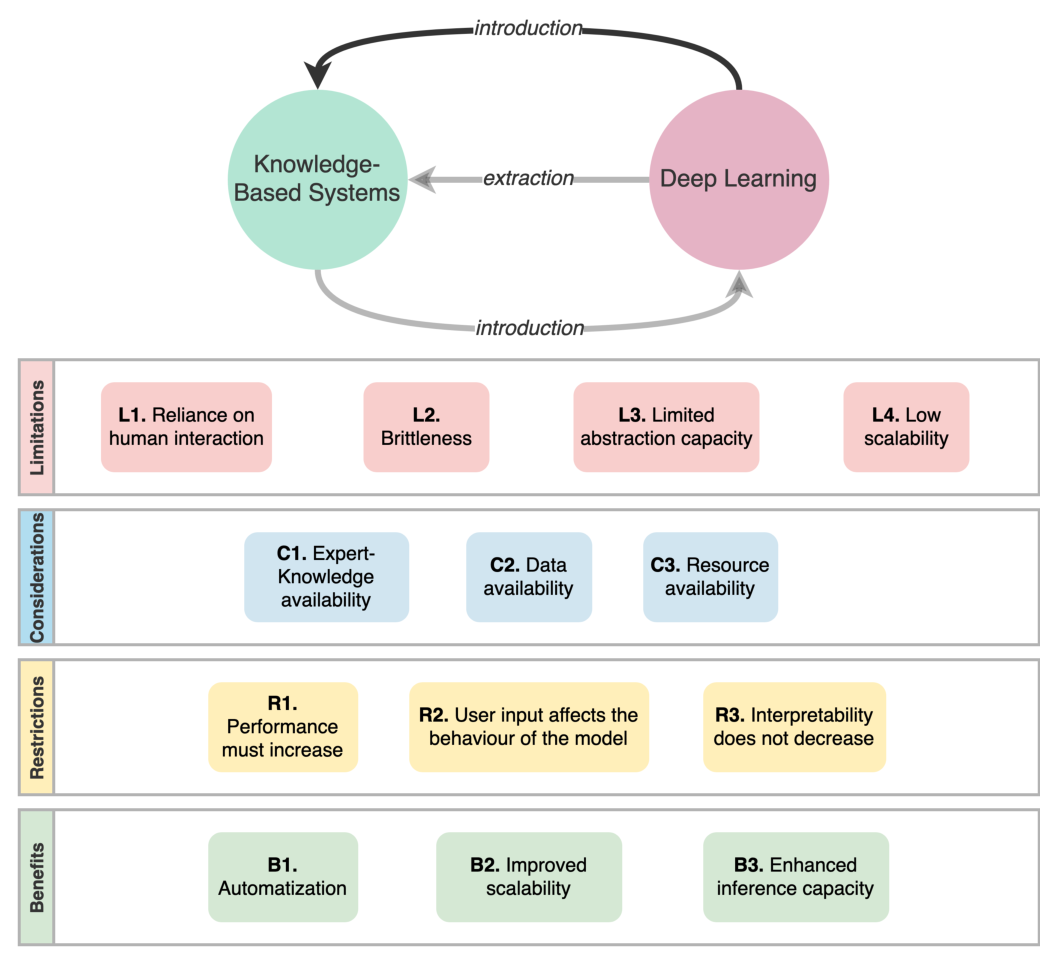
\includegraphics[width=\linewidth]{5_dlintegrationkbs/figures/DL_intro_KBS.eps}
    \caption{Overview on the Insertion of Deep Learning into a Knowledge-Based System.}
    \label{fig:overview_dl_kbs_intro}
\end{figure}
In the second integration approach, the KBS is the primary model, while DL serves as a supporting element. Figure \ref{fig:overview_dl_kbs_intro} outlines the design parameters for the introduction of DL into KBS.
\subsection{Limitations}
\begin{enumerate} [start=1,label={\bfseries L\arabic*.}]
    \item \textbf{Reliance on human interaction.} \label{dl_intro_kbs_L_human} While some KBS behave autonomously, the majority of them have expert knowledge as their cornerstone.  Expert knowledge can not be automatically elicited, as it comes directly from human users. Moreover, the implication of human users within the KBS may not be only limited to their deployment, but can also be required for validation, extension, and maintenance. 
    \item \textbf{Brittleness.}\label{dl_into_kbs_L_brittle} In DL models, brittleness was a result of the nonexistence of restrictions. In the case of KBS, prediction instability is induced by the use of discrete formalization. These hardcoded generalizations about data hinder the capture of exceptions, making the system volatile to the presence of noise and data changes.  
    \item \textbf{Limited abstraction capacity.}\label{dl_into_kbs_L_abstraction} Most KBS models rely on formal representations to reason over input data. Some of these representations have a probabilistic background (e.g. Bayesian Networks) that enables some degree of uncertainty on the predictions of a given input. However, even probabilistic KBS models experience difficulties when processing inputs that do not fall within the specified representations. Moreover, the number of formalizations required to cover over all the elements in the KB are subject to combinatorial explosions, limiting its reasoning capability.
    \item \textbf{Low scalability.}\label{dl_into_kbs_L_scalability} KBS, specially rule-based models, grow proportionally to the size of the KB. Additionally, generating knowledge bases for KBS is an expensive and tedious process. There are approaches to automatically extract KBs from unstructured data, but they still require expert supervision to ensure the correctness of the mined information. Subsequently, the scalability of KBS is remarkably limited.  
\end{enumerate}

\subsection{Considerations}
\begin{enumerate} [start=1,label={\bfseries C\arabic*.}]
    \item \textbf{Expert-Knowledge availability}\label{dlintrokbs_C_expert} As outlined in \ref{dl_intro_kbs_L_human}, most KBS rely on expert knowledge for its construction and maintenance. Regardless of whether DL is integrated within the KBS, expert knowledge must be guaranteed before developing the KBS. Moreover, its availability should be extended to the maintenance stage to ensure that the system behaves correctly.
    
    \item \textbf{Data availability}\label{dlintrokbs_C_data} KBS do not require an elevated amount of data. DL models, however are data hungry (as outlined in \ref{kbsintrodl_L_data_hungry} of KBS introduction into DL). Before integrating DL within a KBS model, it must be ensured that enough data for DL model training is available. 
    
    \item \textbf{Resource availability}\label{dlintrokbs_C_resource} Opposite to DL models, KBS do not require powerful computational resources to run. Instead, KBS models need to store the KBs and, in some approaches, the reasoning representations. The integration of KBS and DL in this context poses two challenges, as both storage and computational resources need to be assured for both elements to function.
\end{enumerate}
\subsection{Restrictions}
\begin{enumerate} [start=1,label={\bfseries R\arabic*.}]
    \item \textbf{Performance must increase.} \label{dlinstrokbs_R_performance} The inclusion of DL in a KBS carries an computational cost. Therefore, the resulting hybrid approach is expected to show a performance improvement with respect to the baseline KBS for the integration to be cost-effective. 
    
    \item \textbf{User input affects the behaviour of the model.}\label{dlintrokbs_R_user} User input is indispensable for KBS models (\ref{dl_intro_kbs_L_human}). While it can be perceived as limiting, it ensures the correct behaviour of the KBS. The impact that external input has on the behaviour of the system should remain with the introduction of DL, correcting not only the behaviour of the KBS but also of the DL.
    
    \item \textbf{Interpretability does not decrease.}\label{dlintrokbs_LR_interpretability} One of the main assets of KBS is their high interpretability. KBS are designed to both integrate external input and produce outputs whose inference process can be understood by humans. DL models, on the contrary, behave as black-boxes. Therefore, their integration should be performed in a way that does not obscure the inference process, so that it can still be understandable.
    
\end{enumerate}
\subsection{Benefits}
\begin{enumerate} [start=1,label={\bfseries B\arabic*.}]
    \item \textbf{Automatization.}\label{dlintrokbs_B_automatization} As outlined in \ref{dl_intro_kbs_L_human}, human interaction (specially expert knowledge) is essential for generating and maintaining KBS. DL models, on the contrary, have a mostly autonomous behaviour. Therefore, the introduction of DL in KBS may serve to automatize some of the steps required to deploy, maintain and validate KBS, reducing the need of human intervention.
    
    \item \textbf{Improved scalability.}\label{dlintrokbs_B_scalability} KBS are limited in terms of scalability due to their reliance on human intervention (\ref{dl_into_kbs_L_scalability}). The inclusion of DL modules within the KBS, as well as automatizing some tasks, can improve the scalability of the system. For example, extracting formal representations from a set of unstructured data.
    
    \item \textbf{Enhanced inference capacity.}\label{dlintrokbs_B_inference} KBS models struggle with capturing non explicit exceptions from data (\ref{dl_into_kbs_L_brittle}. DL models infer abstract patterns from data, capable of assigning an output for any input, even for outliers. Moreover, DL models only require samples of previously unseen inputs to infer new feasible patterns for their correct classification (\ref{dl_into_kbs_L_abstraction}). The introduction of DL modules into a KBS could not only enhance its abstraction capacity, but improving the reasoning of the model on outlier elements.

\end{enumerate}


\section{Deep Learning Powered Case-Based Reasoning for Medical Document Processing}\label{5_sec:dl_powered_kbs_medical}
Case-Based Reasoning (CBR) integration with DL is one of the scenarios depicted in Section \ref{sec:sota_dl_kb_intregration}. As denoted, CBR is often posed as an alternative to rule-based systems. This Section presents a use case on the medical domain, where DL modules are injected into a CBR model. One of the most interesting conclusions of the systematic review in \cite{amador_systematic_review_2019} is the predominance of interpretable, knowledge-based systems in the medical domain. Explainability was rated as one of the key features of these models, thus showing its relevance for its application to this domain. Therefore, the CBR acts as the primary model in this scenario, ensuring that the final hybrid DL-powered approach remains interpretable. 

\begin{figure}[t]
    \centering
    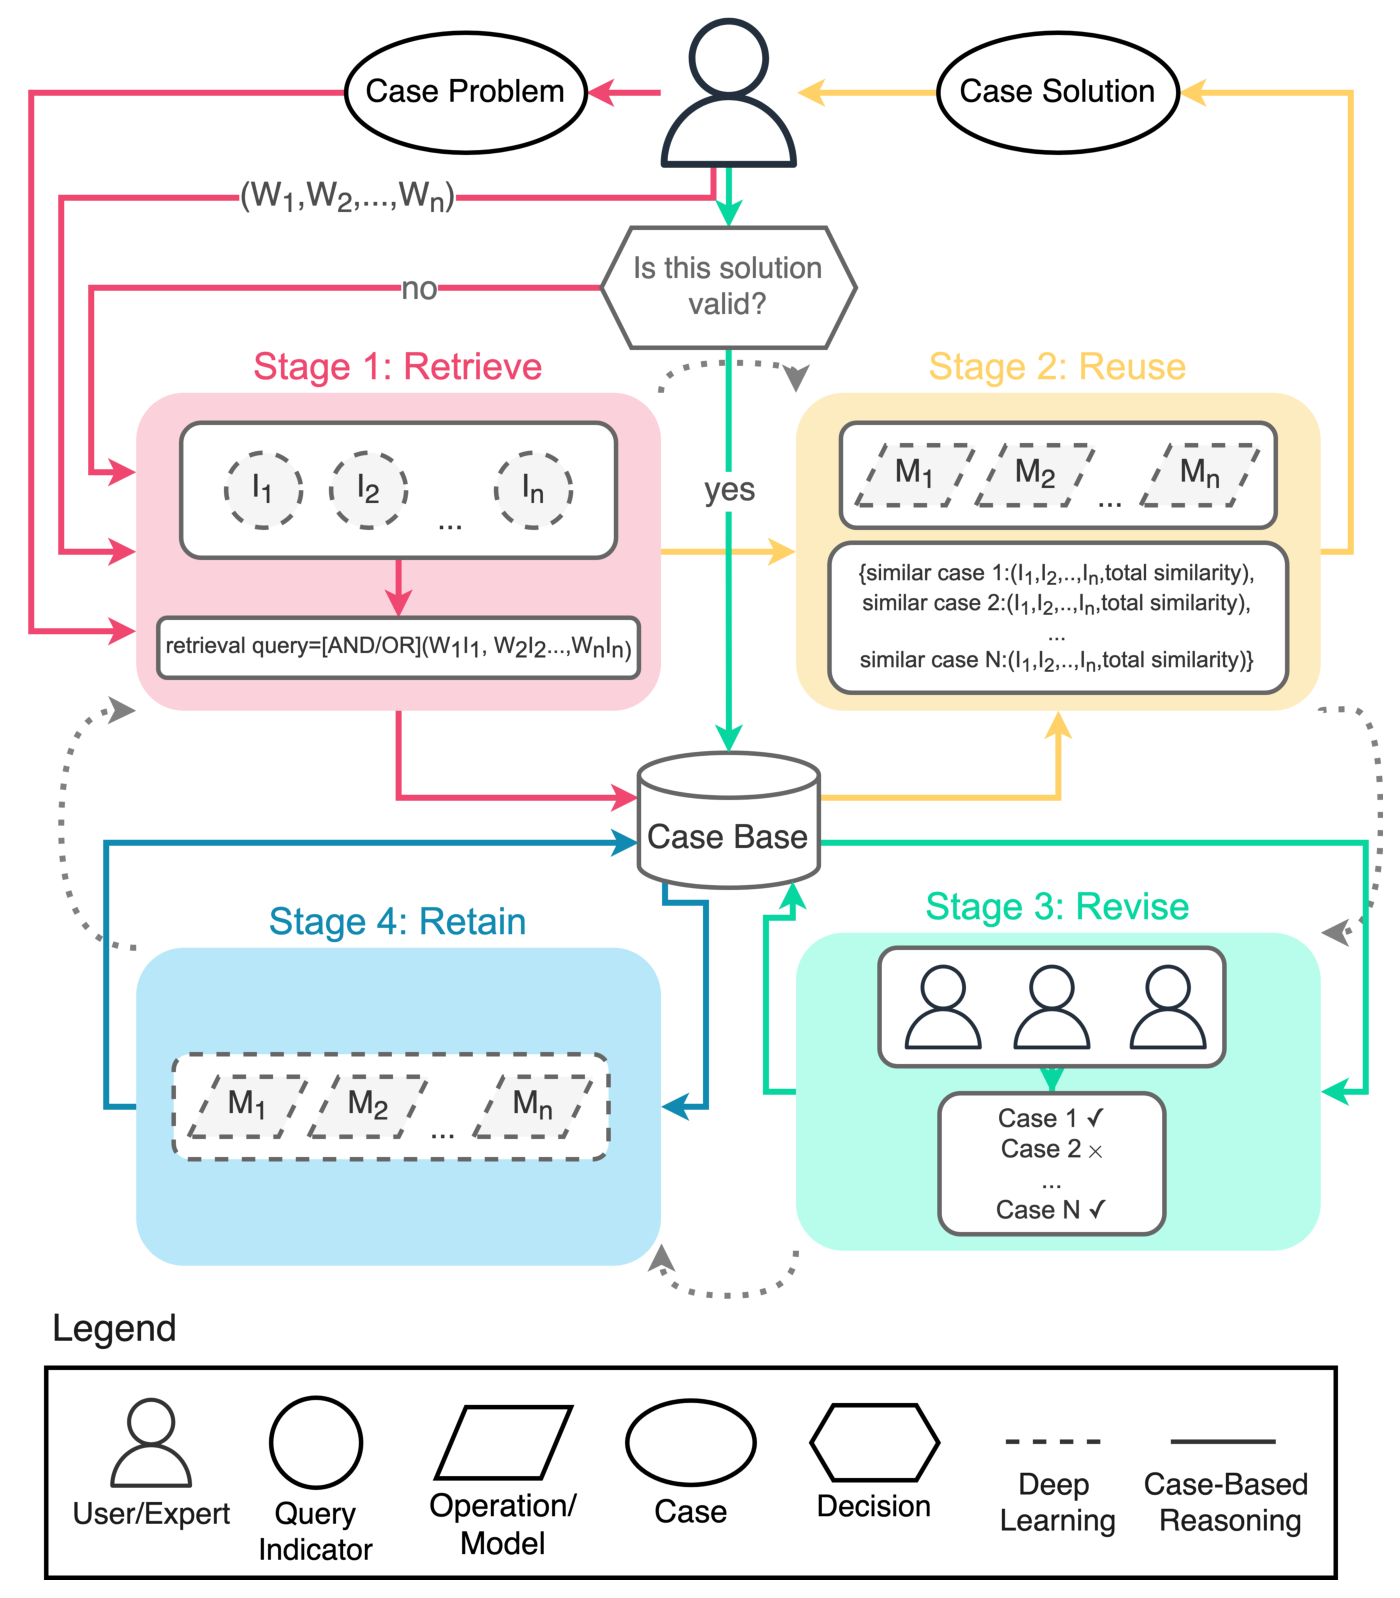
\includegraphics[width=.8\linewidth]{5_dlintegrationkbs/figures/Overview_CBR_DL.eps}
    \caption{Overview of the Deep Learning powered Case-Based Reasoning Model.}
    \label{fig:overview_CBR_DL}
\end{figure}

Figure \ref{fig:overview_CBR_DL} depicts a general overview of the proposed hybrid model. Dashed line denotes the elements where DL can be introduced so that the integrity and interpretability of the CBR model is not compromised, but a performance enhancement is induced. The proposed framework provides assistance in the generation of medical reports, as presented in \cite{DBLP:journals/ijimai/Amador-Dominguez21}. It is not devised to replace the behaviour of the expert, but to provide formal corrections, references, and suggestions to improve the final quality of the results. 

CBR behaves cyclically, comprising four stages: retrieve, reuse, revise, and retain. These stages are differentiated in Figure \ref{fig:overview_CBR_DL}, showing the interactions between phases, as well as between the framework and the user. 

\color{purple}

\subsection{Retrieve}\label{5_sec:dl_powered_cbr_retrieve}
The CBR cycle is initiated when the user inputs a new case problem. A case problem can be simply a text draft, or it can include additional relevant information such as images, related terms or references. In the first stage of the CBR cycle, retrieve, the goal is to determine which of the cases stored in the case base have a higher resemblance to the input. A naïve approach to find the existing closest cases is to use a simple K-NN algorithm, where $K$ is the number of cases to retrieve and the selection is purely based on the distance between the input and the existing samples. K-NN offers a straightforward and efficient solution, but it exhibits two shortcomings that hinder its usage: i) the input data may not always be numerical and easy to measure, and ii) the application domain is expert-oriented, so more specific and revised criteria are required to accurately retrieve cases.

While similarity between reports can be measured according to quantitative metrics such as the age of the patient or demographic data, there are no fixed static criteria that enable straightforward comparison. Some metrics may remain static between comparisons, but others may vary between users. The proposed framework uses an indicator-based retrieval algorithm to overcome these issues. Instead of comparing the cases as a whole, the retrieval algorithm evaluates the values of the different indicators for each case. As depicted in Figure \ref{fig:overview_CBR_DL}, the number of indicators is not predefined and can be adapted to fit different case scenarios. For its application in the medical domain, four indicators are identified:
\begin{itemize}
    \item I1. \textit{Image Comparison.} Images are the cornerstone of some medical areas, such as neurology or dermatology. In those fields where pictures provide essential information, they should not be diluted within the text, but treated separately. Several methods for image comparison can be considered, ranging from histogram to feature vector comparison. Convolutional Neural Networks (CNNs) are a potential DL option for this indicator. CNNs are possibly the most robust way to translate images into a fixed-dimensional space. However, simpler, non-DL alternatives can be also applied. Feature matching algorithms, such as SURF \citep{image_surf}, ORB \citep{ORB_image} or KAZE \citep{KAZE_images} are potential interpretable alternatives to CNNs. However, feature matching algorithms are highly sensitive to potential image failures, such as light flashing, and cannot capture finer-grained information. A potential solution for this issue is to combine differently generated vector representations into a unique vector. Once the image is embedded into a single vector, distance-based can be performed to measure the similarity with respect to the existing images.
    
    \item I2. \textit{Document Comparison.} Similar to the previous case, multiple approaches can be considered for document comparison. Non-feature-based methods can perform this task, but their performance is noticeably subpar with respect to that where documents are embedded into a vector space and can be compared using distance-based metrics. Language models such as ELMO \citep{elmo} or BERT \citep{bert} are the preferred choices for document embedding, but simpler methods such as bag-of-words or TF-IDF can also be applied. Despite reducing the computational cost, these methods cannot capture the underlying semantic information, which leads to less expressive representations. Regarding embedding comparison, different paradigms can be considered, depending both on the type of documents to compare and their purpose. In this respect, cosine similarity, word's mover distance \citep{word_mover_distance}, or probabilistic based methods (in which the embedding is converted into a probabilistic distribution) are suitable choices.
    
    \item I3. \textit{Named Entity Comparison.} Named Entity Recognition (NER) is one of the key tasks in the Natural Language Processing area, being particularly relevant in the medical domain. The goal of this task is to detect and label relevant terms within the text, such as people, places, or dates. Its use is particularly extended in the medical domain, where several NER models have been developed to identify specific medical terms within texts such as diseases, proteins or drugs. CliNER \cite{cliner}, BioBERT \citep{biobert} or SciBERT \citep{scibert} are examples of clinical NER models. Annotating relevant terms within documents can be an effective tool to detect and retrieve related documents. Therefore, only those cases whose reports contain relevant terms are considered for retrieval, greatly reducing the search scope.
    
    \item I4. \textit{Noise Filtering Criteria.} Additional filtering criteria to discard unfitting cases may be required in addition to the previous indicators. These criteria focus on formatting specifications (i.e. absence of images, language) or content elements (i.e. typos, number of abbreviations unidentified). Filtering criteria can be customized to be as restrictive as necessary. 
\end{itemize}

For each indicator, the user can establish a threshold value. Indicators can be treated either conjunctively or disjunctively, according to the user's preference. These criteria are then translated into a search query, which is executed to retrieve the specified number of cases which meet the user-provided constraints.

\begin{lstlisting}[captionpos=b, breaklines=true, float=tp,floatplacement=tbp, caption=Example of a retrieval query., label=lst:lst_query_sample,basicstyle=\ttfamily,frame=single]
   query={ I1>=0.85, I2>=0.7, I3=[Pulmonary Disease,  Pneumonia], I4=[lang= 'en', identified_abbrv_rate>= 0.9 ], N=5, operation= 'OR'}
\end{lstlisting}

Listing \ref{lst:lst_query_sample} is an example of a retrieval query. This query specifies the retrieval of the top 5 cases that either:
\begin{itemize}
    \item Include images that are similar to at least 85\% to those present in the input report.
    \item Medical reports are similar in at least 70\%.
    \item Contain medical terms \textit{pulmonary disease} and \textit{pneumonia}.
    \item Are written in English, and at least 90\% of the detected abbreviations have been disambiguated.
\end{itemize}

Cases that meet the retrieval criteria are ordered in descending order according to their cumulative similarity across the indicators. The top \textit{k} cases demanded by the user are returned.

\subsection{Reuse}\label{5_sec:dl_powered_cbr_reuse}
As depicted in Figure \ref{fig:overview_CBR_DL}, the reuse stage starts once the top \textit{k} similar cases are retrieved. A brief summary on the results of the indicators of each selected case is provided to the user to keep the transparency of the model. From the instances retrieved in the previous stage, different operations are performed to obtain helpful, relevant information to assist the user in the generation of the report. Different modules perform several operations, as depicted in Figure \ref{fig:overview_CBR_DL}. As denoted by the dashed line, these modules can be implemented using DL. In the present case scenario, four modules are identified:
\begin{itemize}
    \item M1. \textit{Formatting Module.} Readability is one of the most prominent features of any written document. Syntactic cohesion, as well as correct formatting are some of the elements that make a document readable. In the case of medical documents, while there may exist differences between specialities, there is usually a fixed structure in which the data is presented. From a general standpoint, a medical report comprises four main sections:
    \begin{itemize}
        \item \textit{Indication.} A brief introduction to the report, giving superficial information about the patient and the observed symptoms.
        \item \textit{Comparison.} References to previous reports of the same patient.
        \item \textit{Findings.} Extensive information about the potential causes of the symptoms, as well as additional observations about the patient.
        \item \textit{Impression.} Conclusions and diagnosis.
    \end{itemize}
    Therefore, this module generates a structured, paragraphed version of an input report in raw format.
    
    \item M2. \textit{Scoring Module.} The system provides the user a validity score indicating whether the report, in its current form, is readable and understandable. This score can be either a simple binary value (valid or nonvalid), a star-score method, or a finer decimal score.
    
    \item M3. \textit{Disambiguation Module.} Abbreviations are recurrent in the medical domain due to the existence of a considerable number of complex compound terms. While most of these abbreviations may be universal and understandable by any professional, some can still be non-understandable for a regular reader. Therefore, the goal of this module is to detect the existing abbreviations within the text and offer disambiguations for them. While this may increase the extension of the document, it also improves its readability noticeably.
    
    \item M4. \textit{Term Recommendation Module.} As previously stated, NER is a critical challenge in the medical domain. NER models can accurately detect relevant terms in a text and groupd them in a fixed set of categories. These categories are usually related and, subsequently, the corresponding terms. For example, given a report about a patient with a pulmonary disease, terms such as (\textit{pneumonia,disease}) and \textit{(chest x-ray,test)} may be frequently featured together. This module mines these correlations between terms, and suggests their inclusion to the user. NER is performed over the output cases of the retrieval phase, obtaining a set of categorized terms. This set of terms is then flattened, cleaned and presented to the user. In the aforementioned example, if the user is writing a report containing the term \textit{pneumonia}, but not \textit{chest x-ray}, the system may suggest the inclusion of this term due to its existent correlation.

\end{itemize}

As users play a key role in CBR models, the recommendations and suggestions offered by the framework are not final. Instead, the user decides which of the suggestions and corrections are to be applied to the input report. When the user approves the final state of the report, a new case is generated and stored in the case base, using the initial report as the problem and its corrected version as the solution. Case bases are not immediately incorporated into the case base, but marked as \textit{to be validated} until an expert validates them.

\subsection{Revise}\label{5_sec:dl_powered_cbr_revise}
A new case is generated once the user effectuates the applicable suggestions to the report. New cases are not automatically included in the case base for future iterations of the cycle, as they may include errors that can negatively affect the behaviour of the system. Moreover, if the system stores unreliable cases into the case base without any revision, they may be retrieved in the subsequent iterations, generating erroneous suggestions and corrections. An intermediate step is required to ensure that all cases stored in the case base are useful and relevant. 

In the revise stage, a panel of experts manually checks the upcoming cases, rating and correcting them. The scores provided by the experts must be coherent with the grading system used by the scoring module. Therefore, if the scoring module uses binary scoring, experts must extend this criterium to new cases.


\subsection{Retain}\label{5_sec:dl_powered_cbr_retain}
One of the main challenges of CBR systems is how to efficiently manage the case base. Ideally, the case base should be optimized, containing the minimum number of relevant cases that ensure the maximum coverage. Non-valid cases are not stored in the case base, but are stored separately to serve as negative samples for the scoring module. 

New cases are being regularly introduced into the case base, subsequently unchaining a reaction within the system. CBR models improve with the inclusion of new cases, which keeps them usable and updated throughout time. In the retain stage of the cycle, besides performing case base maintenance, reuse models are updated and checked. Reuse model updates can be either a replacement for the modules, such as switching from regular expression or rule-based systems (when the number of cases is limited) to DL models when the available data increases. 

\section{A Hybrid Case-Based Reasoning and Deep Learning Framework for Radiological Report Recommendation}\label{5_sec:raidologist}

This Section presents an implementation of the general framework depicted in Figure \ref{fig:overview_CBR_DL} focusing specifically on radiological reports. This context presents a challenging scenario, as both image and textual information are equally relevant. Figure \ref{fig:raidologist_data_flow} showcases the data flow of the implementation, instantiating the different components described in Section \ref{5_sec:dl_powered_kbs_medical}. The execution steps of one full iteration of the cycle are also denoted.

\begin{figure}[t]
    \centering
    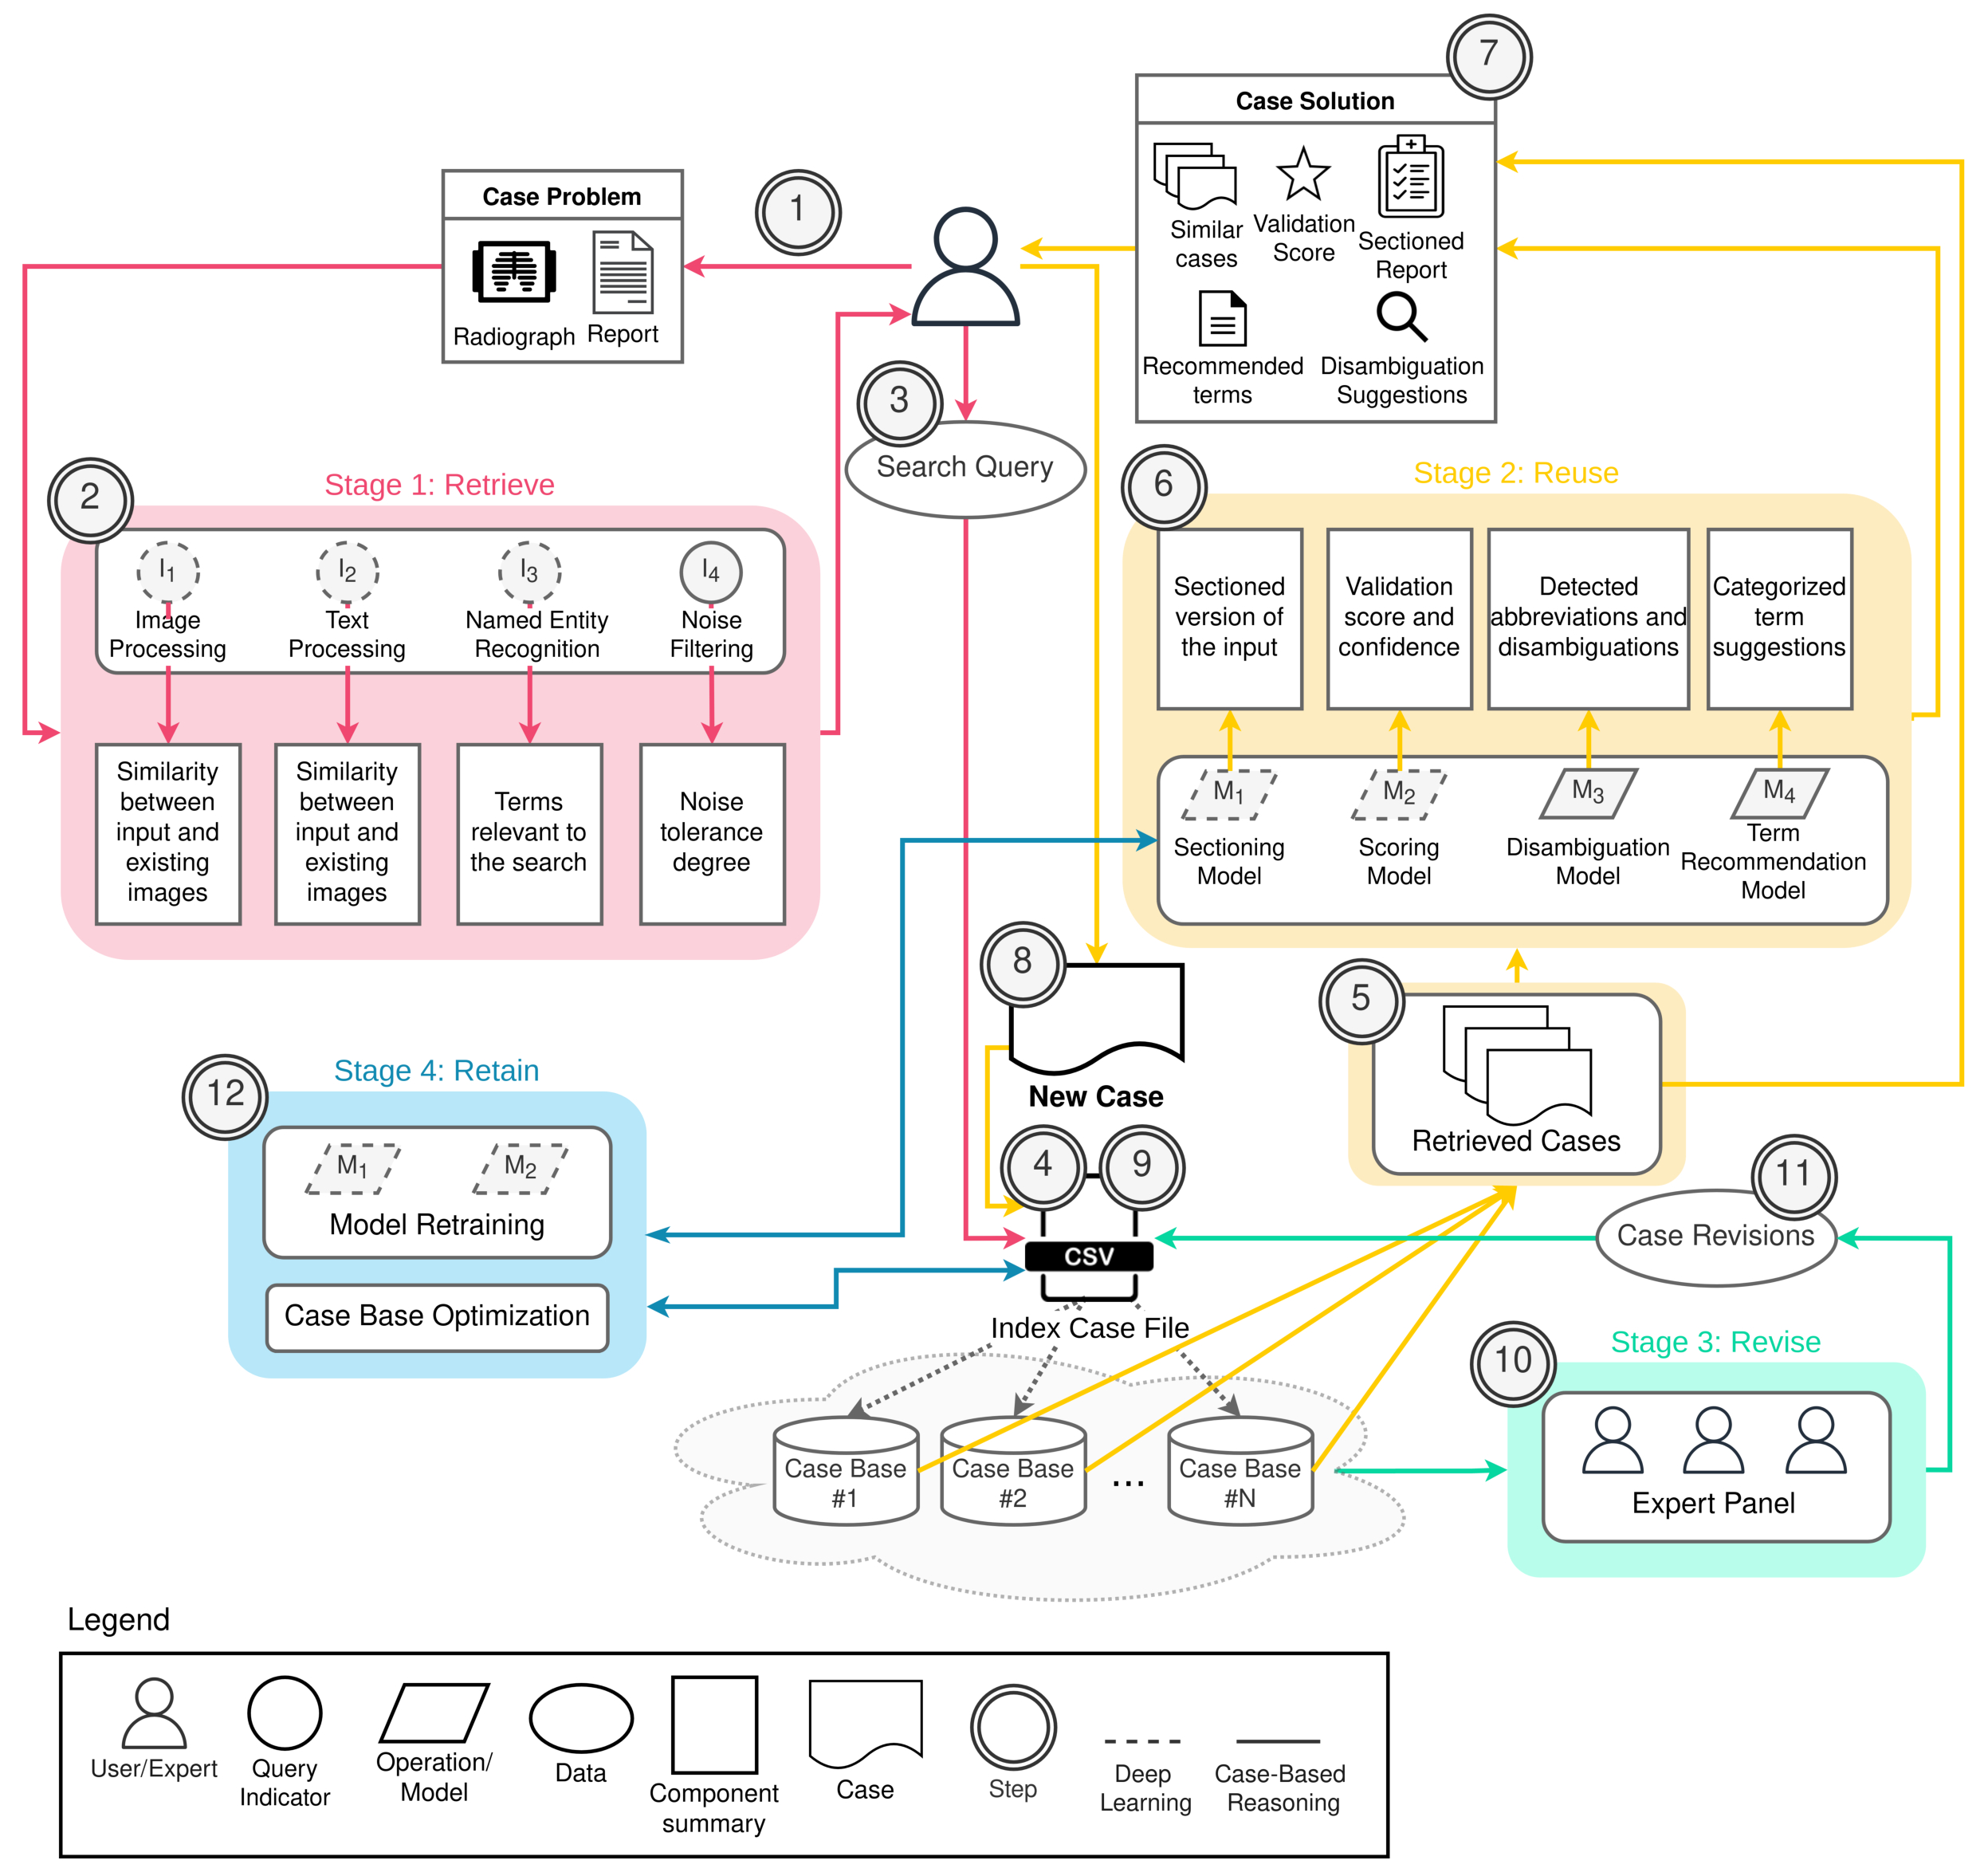
\includegraphics[width=\linewidth]{5_dlintegrationkbs/figures/raidologist_flow.eps}
    \caption{Data flow of the r.AID.ologist framework.}
    \label{fig:raidologist_data_flow}
\end{figure}

The framework is implemented as a four-layered software architecture. Some issues must be addressed before defining the specific components of the proposed hybrid model for the given task, such as data management or storage mechanisms. Indexed storage is employed to deal to efficiently manage the constant growth of the case base while still allowing for efficient retrieval. In the proposed storage, cases are saved either in a distributed or centralized schema and referenced in an index file. The index file contains each case's location and its respective indicators which are computed beforehand, accelerating the retrieval process. 

In the radiology domain, a case is usually composed by one or more radiographs and a brief text summarizing the most relevant findings on the images, alongside additional information about the patient. These are the two minimal elements required to define a case, but additional information can be provided, such as relevant terms, regions of interest, or specific abbreviations. 

The retrieve stage begins when the user inputs a new problem into the system. The case indicators of the input problem are computed as follows:

\begin{itemize}
    \item I1. \textit{Image Comparison.} In radiology, images are black and white radiographs, thus not exhibiting much variation between samples. Convolutional neural networks generate embeddings capable of capturing the subtle differences between radiographs, enabling an accurate comparison between them. A feature detection algorithm is also included to add an additional level of information. KAZE is used to generate fixed-dimension descriptors from a set of key points detected in the image. Key points can be indicated on the image, providing a visualization on the basis on which the images are compared. Both KAZE and CNN vectors are averaged, generating a unique embedding that combines both interpretable and abstract knowledge. Samples are compared via cosine similarity over the resulting embedding.
    
    \item I2. \textit{Report Comparison.} A clinical NLP model is used for this task. This pretrained DL model provides embeddings at word, sentence, and document level. Document embeddings are used to generate comparable report representations. 
    
    \item I3. \textit{Named Entity Recognition} CliNER is used to compute this indicator. CliNER provides a series of models (Bi-Directional Long Short Term Memory networks) trained over a sizeable clinical corpus, capable of identifying the following entity categories: diseases, treatments, and tests. While simple, this categorization is enough to cover the terms identified in the radiology domain.
    
    \item I4. \textit{Noise Filtering.} The same NLP model from I2 is used for noise filtering. In this context, noise encompasses those tokens in the text that cannot be identified as words. Once the report is processed by the NLP model, a set of conflicting terms is obtained. Noise can then be computed as the proportion of identified tokens with respect to the total number of tokens in the text.
\end{itemize}

These indicators are computed only once per case. The user is then inquired for the retrieval query parameters: threshold values of each indicator, the combination paradigm (conjunctive or disjunctive), and the number of cases $k$ to retrieve. The threshold values are reformulated in a human-readable format, as depicted in Figure \ref{fig:raidologist_data_flow}. For example, a valid inquiry for the value of I2 (report comparison) would be: \textit{what is the minimum similarity acceptable between the current and the existing reports?}. Queries must be clearly presented and understandable to the user, as they condition the behaviour of the model during the retrieve phase.

After the search query is generated by the user, a comparison between the current problem and the existing cases is performed. The use of indexed storage enables a fast comparison, as the indicator values of the cases contained in the index file can be directly compared to those of the input. Therefore, a case is only fully retrieved from the case base if it meets the query conditions. A summary of each indicator's similarity metrics is included along each case. 

In the reuse phase, a tailored solution for the input case problem is generated based on the retrieved cases, alongside with the described formatting modules. The retrieved top $k$ similar cases are also included as part of the case solution, serving as format and content references for potential corrections. The devised case solution contains the following suggestions, which are provided to the user:
\begin{itemize}
    \item \textit{Sectioned version of the report:} A DL model (Bi-Directional Long Short Term Memory) is used for text formatting. Sectioning is treated as a classification problem. Training reports are divided into sentences, and each sentence is labelled according to the section where it is featured. Subsequently, the goal of the model is to predict the section where each sentence fits best. When formatting a new report, sentences are input into the DL model in the same order as they appear in the text to avoid content permutations.
    
    \item \textit{Potential disambiguations for text abbreviations:} After computing indicator I4, a list of unidentified tokens is obtained. This set not only comprises noisy entries, such as misspellings, but also abbreviated terms. These tokens are then consulted in the medical terminology SNOMED-CT, seeking to obtain the best applicable term whenever possible.
    
    \item \textit{Case validation score and confidence value:} A binary scoring system is employed to categorize cases between valid and invalid. A DL model composed by a language modelling model in combination with a random forest classifier is used to score the cases, using the cases already validated by the experts in the revise section as training data. While the score assigned to a given case is not final until it has been revised by the experts, it can provide a reference to the user on whether the report on its current state would be suitable for approval. 
    
    \item \textit{Suggested related terms per category:} CliNER is applied to the content of the top $k$ retrieved cases, extracting a set of terms categorized into three types: disease, test, and treatment. Duplicate entries are removed, and the resulting categorized term list is presented to the user.
\end{itemize}

The case solution generated after the reuse phase is then presented to the user, who decides which of the offered corrections should be implemented. A new case is then generated from the initial problem and the solution implemented by the user with the suggestions of the system. This case will then be stored in a case base and labelled as \textit{to be validated} until the revise phase. Non validated cases are not displayed to the user nor used for reuse until their validation by the expert panel. In the revise phase, the expert panel periodically validates the pending cases. The final validation state of new cases is referenced in the index file, accelerating the posterior retrieval search. 

Usually, invalid cases are deleted from the case base, as they technically do not provide valuable information to the user. However, due to the inclusion of DL models, negative samples are necessary to train and obtain robust scoring models. Moreover, once the scoring model reaches enough maturity, it can replace the expert panel, automatizing this phase. 

The retain stage is triggered under one of the following three conditions: i) the expert panel requires it, ii) it is periodically scheduled, or iii) the number of stored cases reaches an specified number. In this stage, both the scoring and sectioning modules used in the reuse stage are updated with the newly added cases. Periodically scheduled retraining ensures that the model is kept updated, but may be ineffective when the number of cases in the case set is reduced. Case based optimization is also performed in this phase. Case correlation is maximized for optimization to obtain the minimum set of cases that give the maximum coverage. First, a global linking process is conducted amongst cases, computing the top 5 similar cases per instance. Cases that are co-referenced by at least one case are kept in the case base. Unreferenced cases are still considered for training the sectioning and scoring models, but will not be part of the CBR cycle in subsequent iterations.


\section{Experimental Results}\label{5_sec:experimental_results}
The presented implementation of the proposed hybrid model is evaluated to assess its accuracy and performance. Most CBR-based approaches are gauged focusing on their retrieval strategy. The proposed framework relies on user-input queries to refine the retrieval process. Hence, assessing the performance of the proposal based solely on the effectiveness of the retrieval mechanism would not be representative enough, as the success of this stage is highly reliant on user criteria.

Since the implementation context (radiological domain) is highly expert-oriented, accurately evaluating the framework without expert information is not trivial. An alternative evaluation approach capable of quantitatively measuring the performance of the model is devised. Report correction is used to measure the effectiveness of the proposal.

\begin{figure}[t]
    \centering
    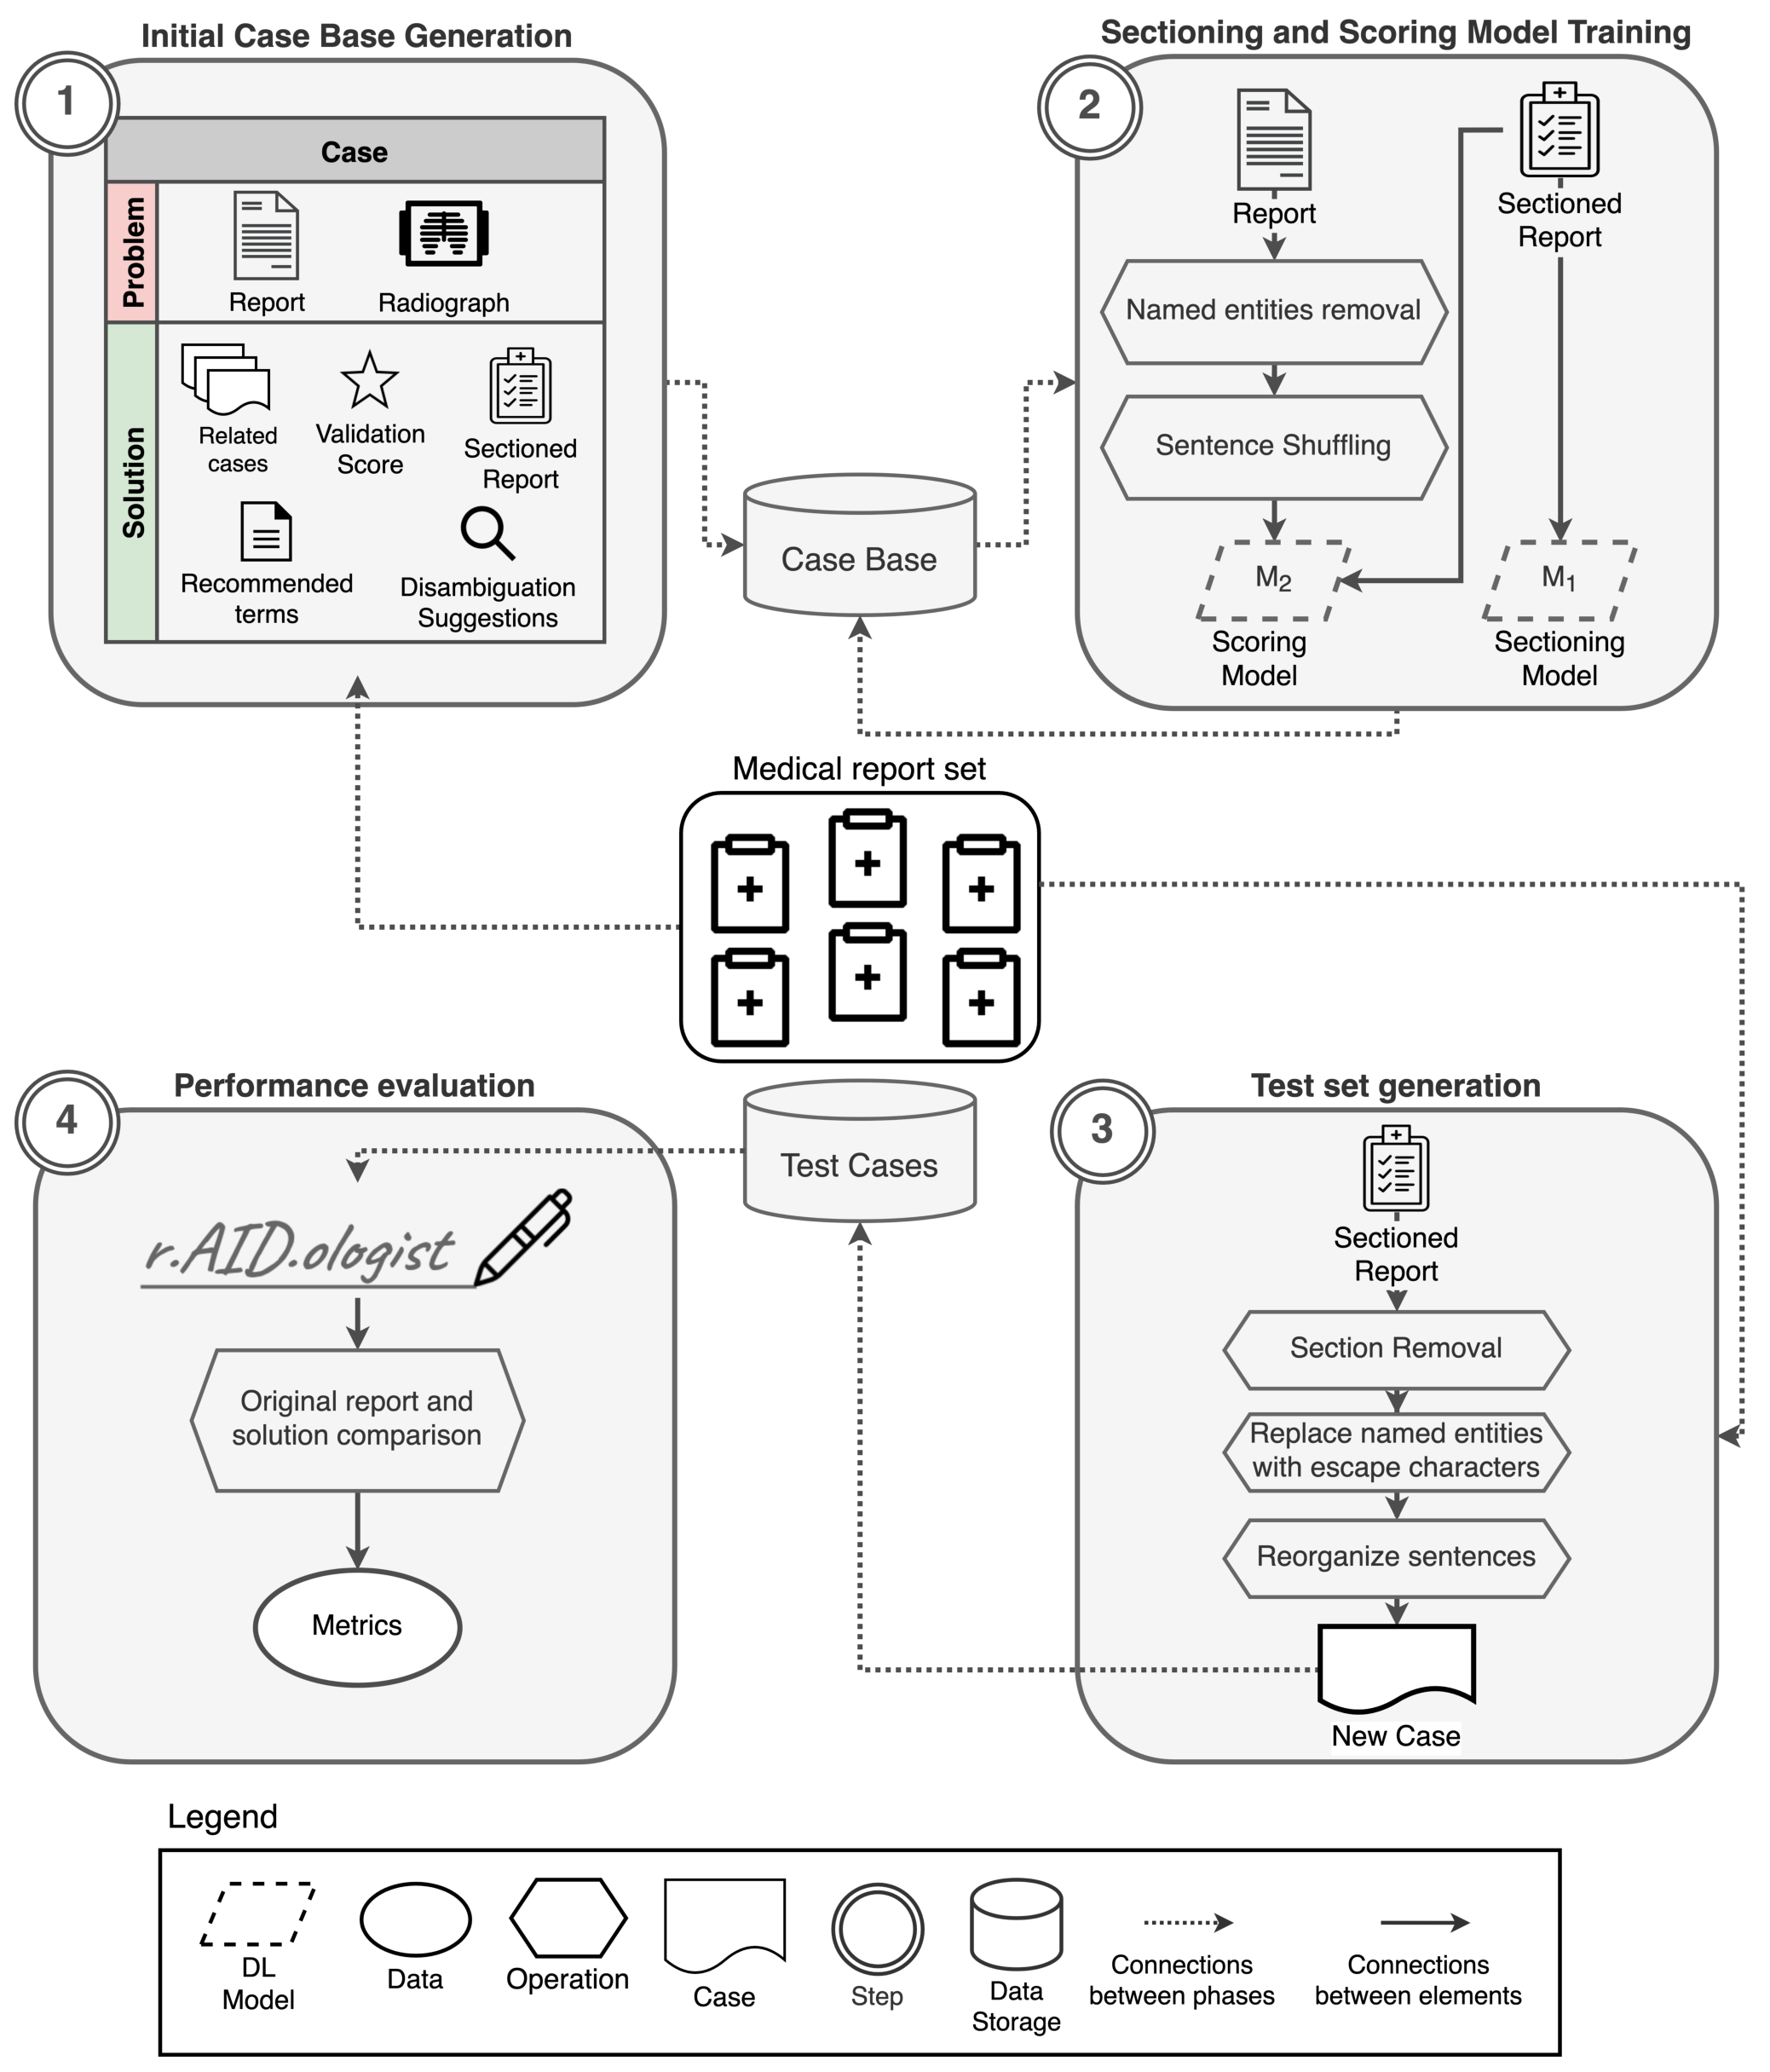
\includegraphics[width=.8\linewidth]{5_dlintegrationkbs/figures/raidologist_experimentation_overview.eps}
    \caption{Overview of the evaluation of r.AID.ologist.}
    \label{fig:overview_experimentation_raidologist}
\end{figure}

Figure \ref{fig:overview_experimentation_raidologist} depicts the four steps of the evaluation process:

\begin{enumerate}
    \item \textit{Initial case base generation.} The case base is the core of any CBR model. In the first step, a set of medical reports is converted into cases, generating the initial case base. Out of all the available medical reports, a sub-sample is selected for later testing. Reports selected for testing are not included in the case base. Each training medical report is then stripped, whenever possible, from its sections to generate the case problem. If a list of named entities or abbreviations is provided alongside the report, these are also included alongside the report in the problem case. If there are radiographs attached to the images, they are included in the case problem as well. The solution to the case is the original medical report. The remaining case solution elements are generated in the following step.
    
    \item \textit{Sectioning and scoring model training.} At this stage, cases contained in the case base are not complete, as they only contain the input problem and one element of the solution (the sectioned report). However, the original and corrupted version of the report are enough to properly train both the sectioning and scoring models. Cases contained in the case base are divided following a 80/20 proportion into two sets: training and validation. The same scoring and sectioning models described in Section \ref{5_sec:raidologist} are used in the evaluation. The sectioning model is trained using case solutions, where each report is split into sentences, and each sentence is labelled according to the section where it was featured. In the scoring model, both the problem and solution of the case are required, as this model feeds positive and negative samples. Case problems comprise the negative sample set, while case solutions are used for its positive counterpart. Section removal and sentence shuffling are also applied for further corruption. Once both sectioning and scoring models are trained, the scoring model is used to update the validation score of each case on the case base. Named entities, disambiguations and related cases are also updated as described in Section \ref{5_sec:raidologist}.
    
    \item \textit{Test set generation.} Test cases are created from the medical reports sampled for this purpose in Step 1. In the devised evaluation, the effectiveness of the model is computed based on whether, given a corrupted version of the original report, the framework is capable of providing suggestions and corrections whose application leads to a version as similar to the original report as possible. For each element in the test set, the following corruption operations are performed to create the case problems: section removal, named entity replacement by escape characters and sentence shuffling.
    
    \item \textit{Performance evaluation.} Test cases are then processed by the system, which generates a corrected version of the input report. Additionally, a list of recommended terms and potential disambiguations is provided. The corrected version of the input, corrupted report is then compared to the original version. The model should be capable of reorganizing the sentences into sections in a cohesive order, as well as suggesting the introduction of the named entities that were previously stripped from the report. The following metrics are then computed:
    \begin{enumerate}
        \item The validation score provided by the model before and after applying the corrections.
        \item The Levenshtein distance between the original report and the suggested correction.
        \item The proportion of entities detected on the original reported whose inclusion is suggested.
    \end{enumerate}
\end{enumerate}


Two different radiology datasets are considered for evaluation: MIMIC-CXR \citep{mimic-cxr} and Open-I's radiololgy set, ECGEN \citep{openi}. MIMIC-CXR contains medical reports in plain text format, without including any additional information. ECGEN provides both images and named entities alongside the medical report, as well as additional metadata. From each dataset, two initial case bases are generated, composed by 50 and 200 cases, respectively. Cases are generated from a random sampling of reports from each considered dataset. 

\begin{figure}[t!]
    \centering
    \subfigure[ECGEN 50-case set \label{fig:ecgen_validation_50}]{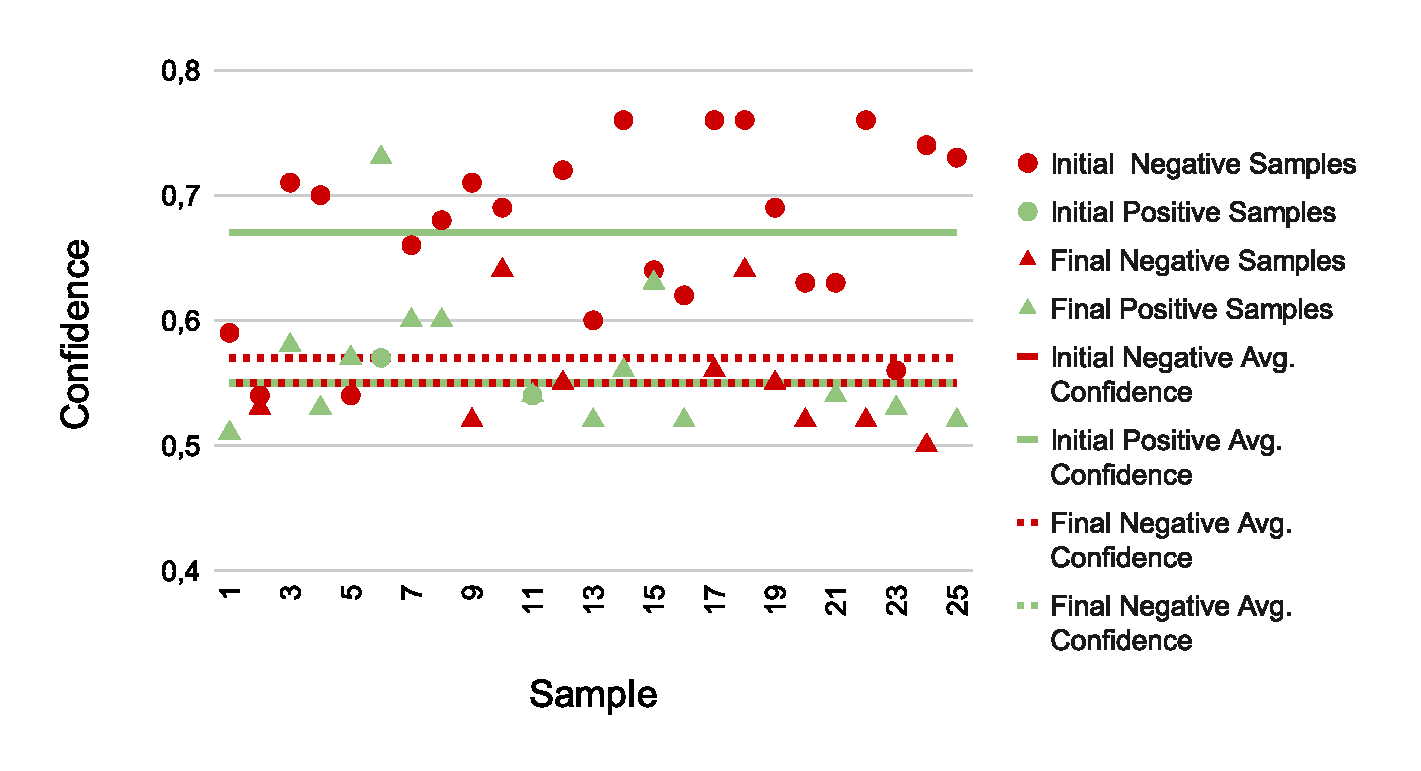
\includegraphics[width=.85\columnwidth]{5_dlintegrationkbs/figures/ecgen_50_validation.eps}}
    \subfigure[MIMIC-CXR 50-case set \label{fig:mimic_validation_50}]{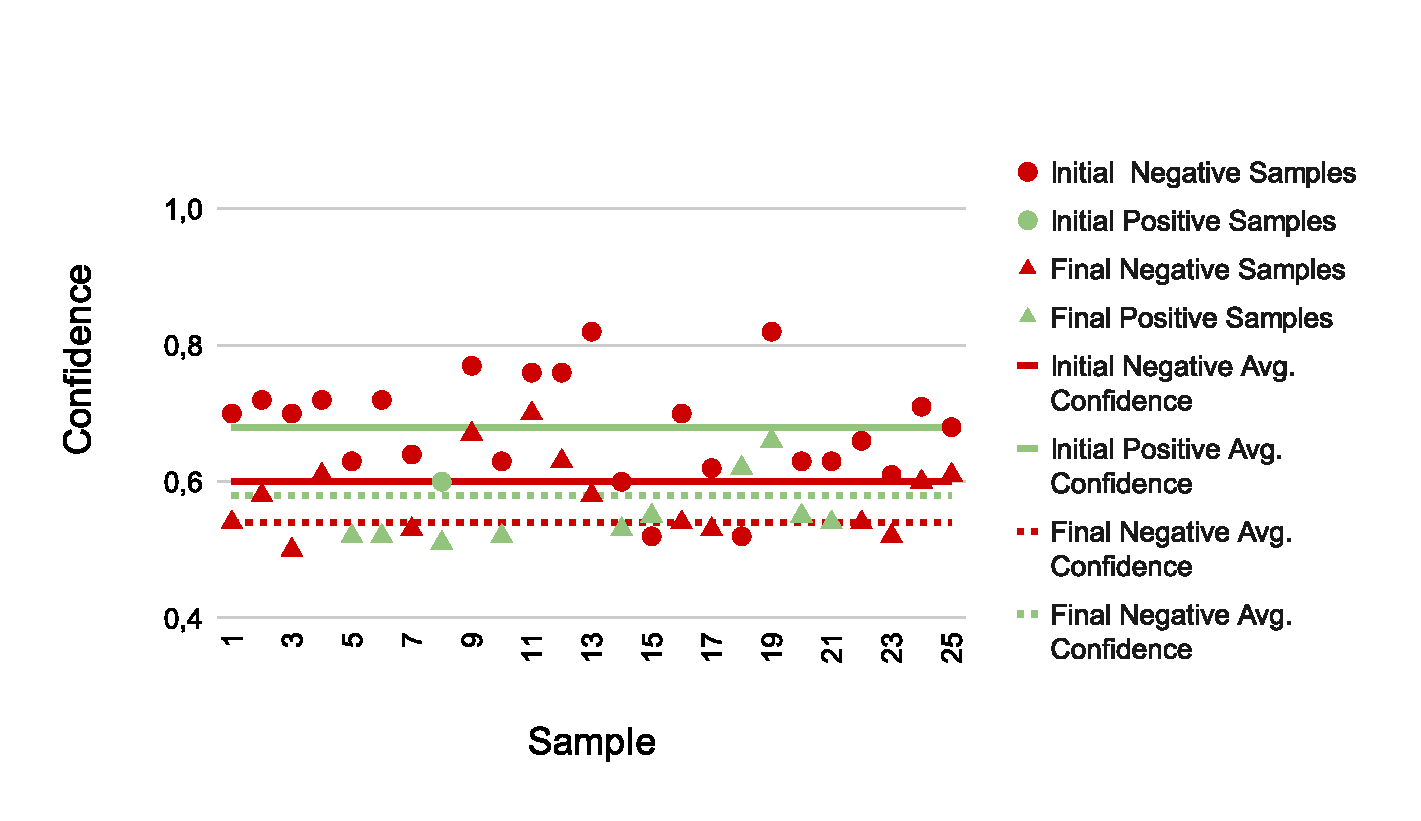
\includegraphics[width=.85\columnwidth]{5_dlintegrationkbs/figures/mimic_50_validation.eps}}
    \caption{Validation status on the 50-case set before and after corrections for the studied datasets.}
    \label{fig:50_set_comparison}
\end{figure}

The initial 50-element case base serves as a baseline to assess the performance of the framework with a limited number of cases. Applying the retain criteria in this scenario may not have any impact, as most cases may be related between them. In the 200-element case base, where the amount of initial cases is four times the size of the prior case base, retain criteria can be successfully applied, obtaining the optimal case base that contains the minimum cases to ensure maximum coverage. The optimal case bases of MIMIC-CXR and ECGEN contain 187 and 90 elements, respectively. Both the baseline and optimal case base are considered for evaluation.

\begin{figure}[t!]
    \centering
    \subfigure[ECGEN optimal case set \label{fig:ecgen_validation_optimal}]{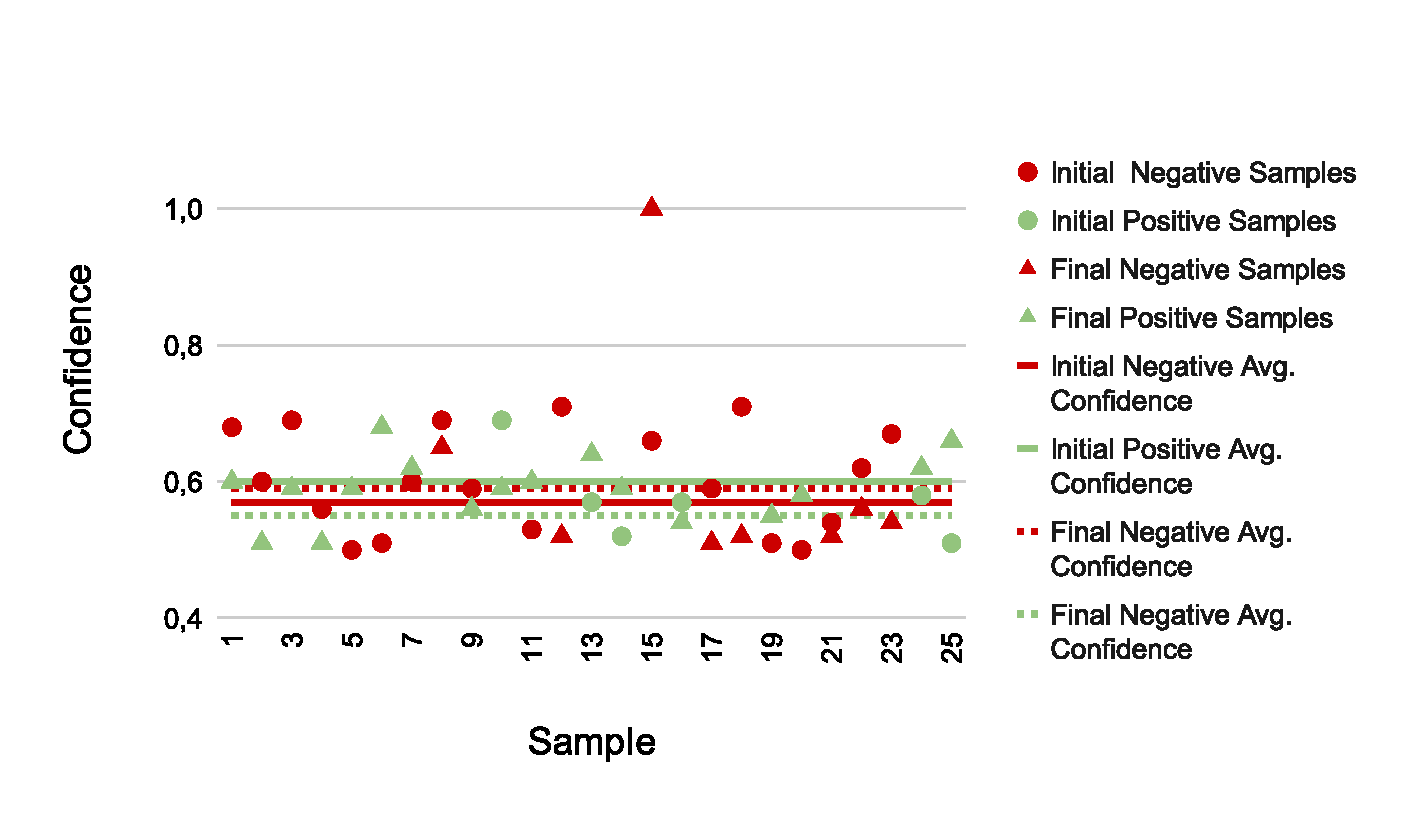
\includegraphics[width=.85\columnwidth]{5_dlintegrationkbs/figures/ecgen_optimal_validation.eps}}
    \subfigure[MIMIC-CXR optimal case set \label{fig:mimic_validation_optimal}]{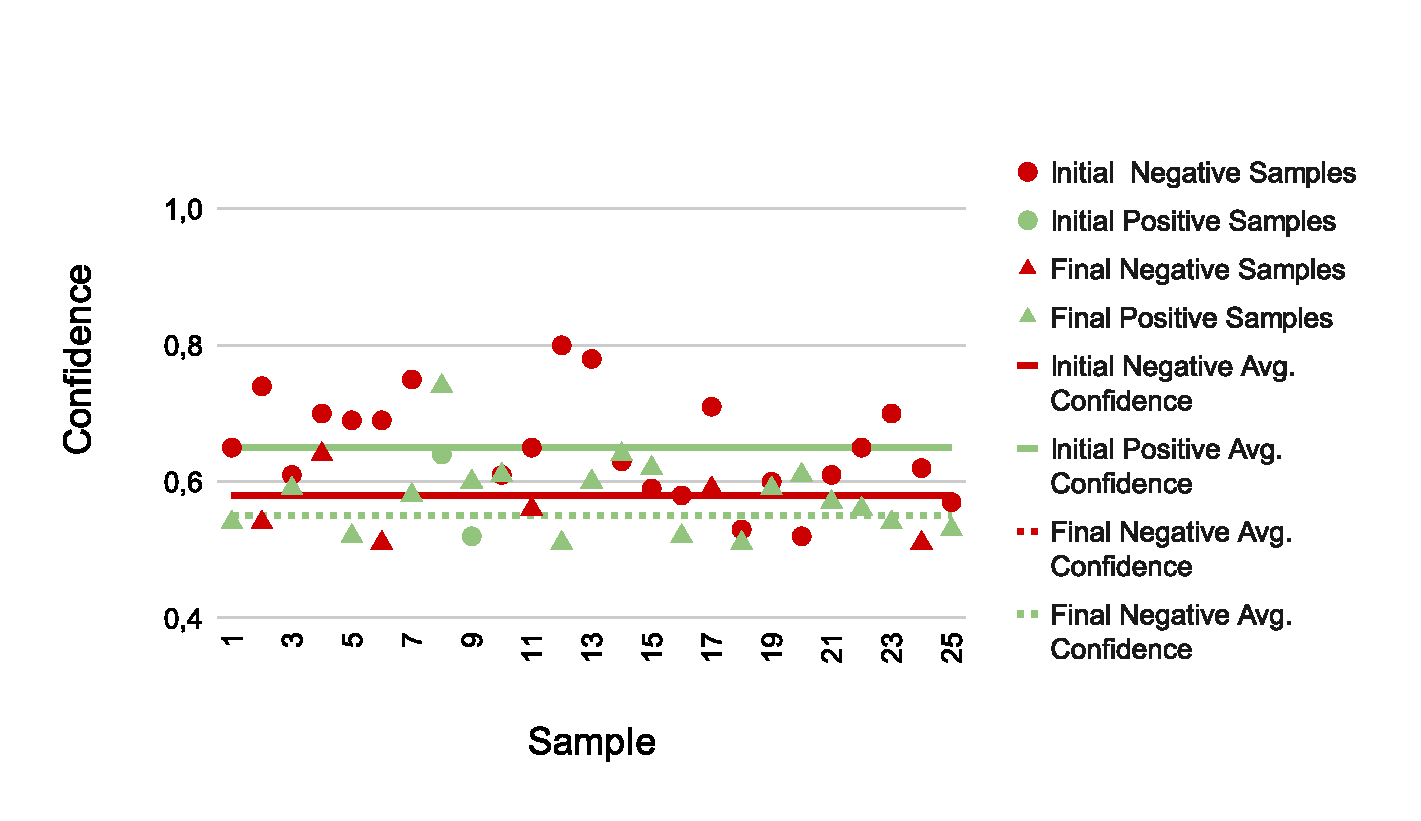
\includegraphics[width=.85\columnwidth]{5_dlintegrationkbs/figures/mimic_optimal_validation.eps}}
    \caption{Validation status on the optimal set before and after corrections for the studied datasets.}
    \label{fig:optimal_set_comparison}
\end{figure}


Figure \ref{fig:50_set_comparison} showcases the performance of the model on the 50-case base per dataset regarding report validation. Despite the limited number of cases in the case base, the framework still achieves noteworthy results, accurately correcting most of the initially invalid cases. In ECGEN (Figure \ref{fig:ecgen_validation_50}) the impact of the correction can be clearly observed, where most of the initial cases that were rated as invalid with a high confidence value turn into valid cases after applying the corrections. For MIMIC-CXR, the improvement is not as noticeable, as some cases are still rated as invalid after applying the system corrections. However, as depicted in Figure \ref{fig:mimic_validation_50}, even in those cases still denoted as invalid after applying the corrections, the confidence value diminishes dramatically. This decrement evidences that, even though the generated solution is still marked as invalid, the system corrections significantly improve the initial report.


As shown in Figure \ref{fig:optimal_set_comparison}, optimizing the case base positively impacts the performance of the model. After optimization, the results are slightly more polarized than in the previous case, as the majority of the initially invalid cases are corrected and validated when processed by the framework. Moreover, the overall confidence values increase with respect to that of the 50-case set, indicating that the scoring model learns to better differentiate valid and invalid cases. Additionally, optimizing the case base also soothes the existing differences in performance. While in the 50-case set the results obtained in ECGEN are slightly better than the ones achieved in MIMIC-CXR, when optimizing both case bases their performances in terms of report validation become fairly similar.

\begin{figure}[t!]
    \centering
    \subfigure[ECGEN \label{fig:ecgen_levenshtein}]{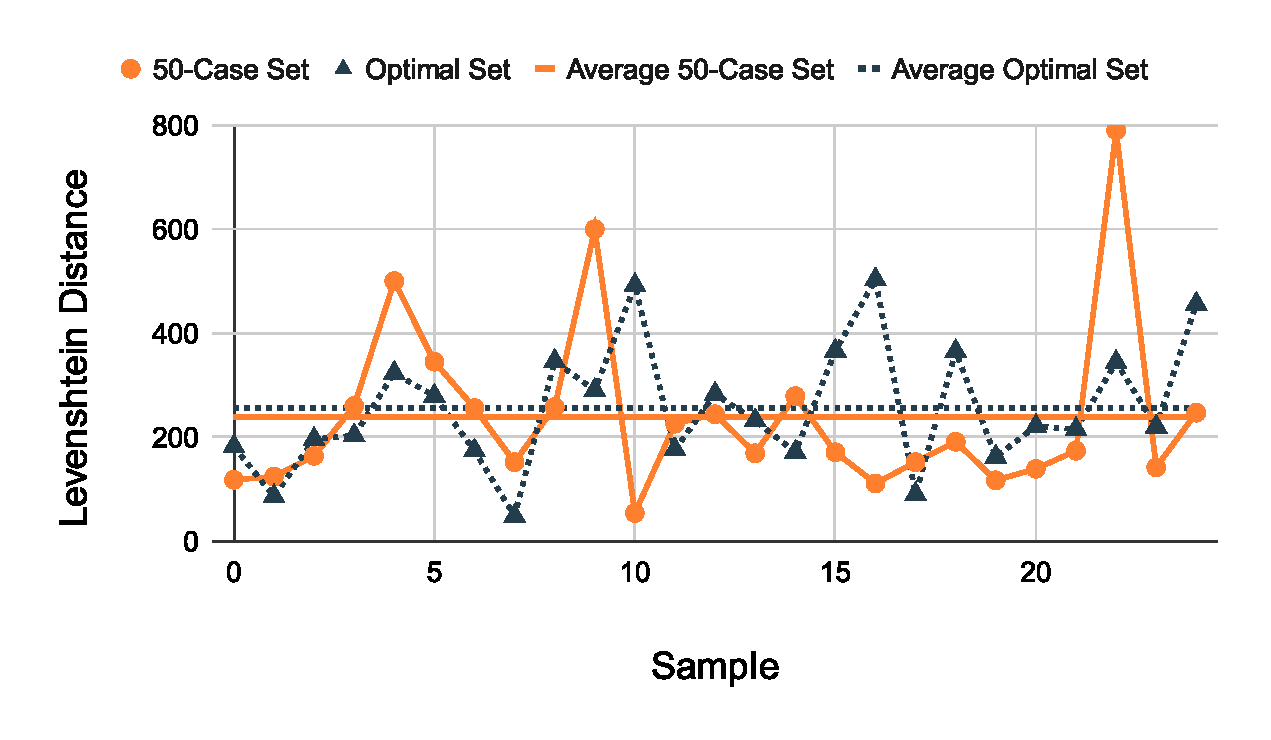
\includegraphics[width=.75\columnwidth]{5_dlintegrationkbs/figures/ecgen_levenshtein.eps}}
    \subfigure[MIMIC-CXR  \label{fig:mimic_levenshtein}]{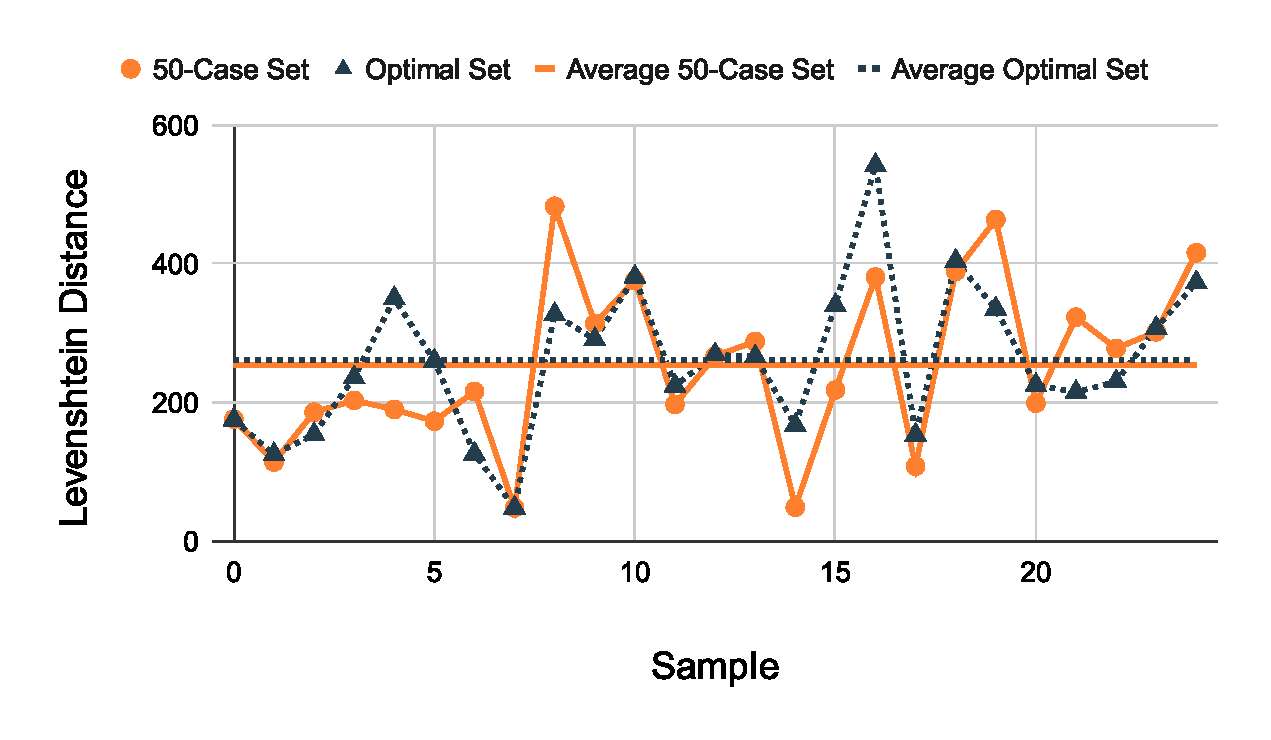
\includegraphics[width=.75\columnwidth]{5_dlintegrationkbs/figures/mimic_levenshtein.eps}}
    \caption{Levenshtein distance per sample on each studied dataset.}
    \label{fig:levenshtein_comparison}
\end{figure}


Levenshtein distance \citep{levenshtein} between each original and corrected report pair is also computed. Different text similarity metrics could be considered for evaluation, such as cosine similarity or Jaccard index. However, none of these metrics consider sentence ordering. As described in Figure \ref{fig:overview_experimentation_raidologist}, test cases are generated by stripping sections, permutating sentence order, and removing named entities. Therefore, even after the corruption process, both the original and corrupted versions of the report are almost equal in terms of content. An order-sensitive metric is required to ascertain the similarity degree between the original and the corrected report. Figure \ref{fig:levenshtein_comparison} reports the Levenshtein distance for each original and corrected report pair on each dataset and case base. Levenshtein distances in ECGEN (Figure \ref{fig:ecgen_levenshtein}) remain reasonably similar in both the 50-case and optimal bases between cases. Similarly, in MIMIC-CXR (Figure \ref{fig:mimic_levenshtein}) the distance between original and corrected reports remains akin. Case based optimization does not induce an additional improvement, as in the validation evaluation. This issue may be alleviated by the introduction of user input. For the evaluation, both the problem and the solution of the cases have been artificially generated. User-corrected reports may be more expressive and richer in content, enabling the identification of more complex correction patterns.

\begin{figure}[t!]
    \centering
    \subfigure[ECGEN \label{fig:ecgen_entities}]{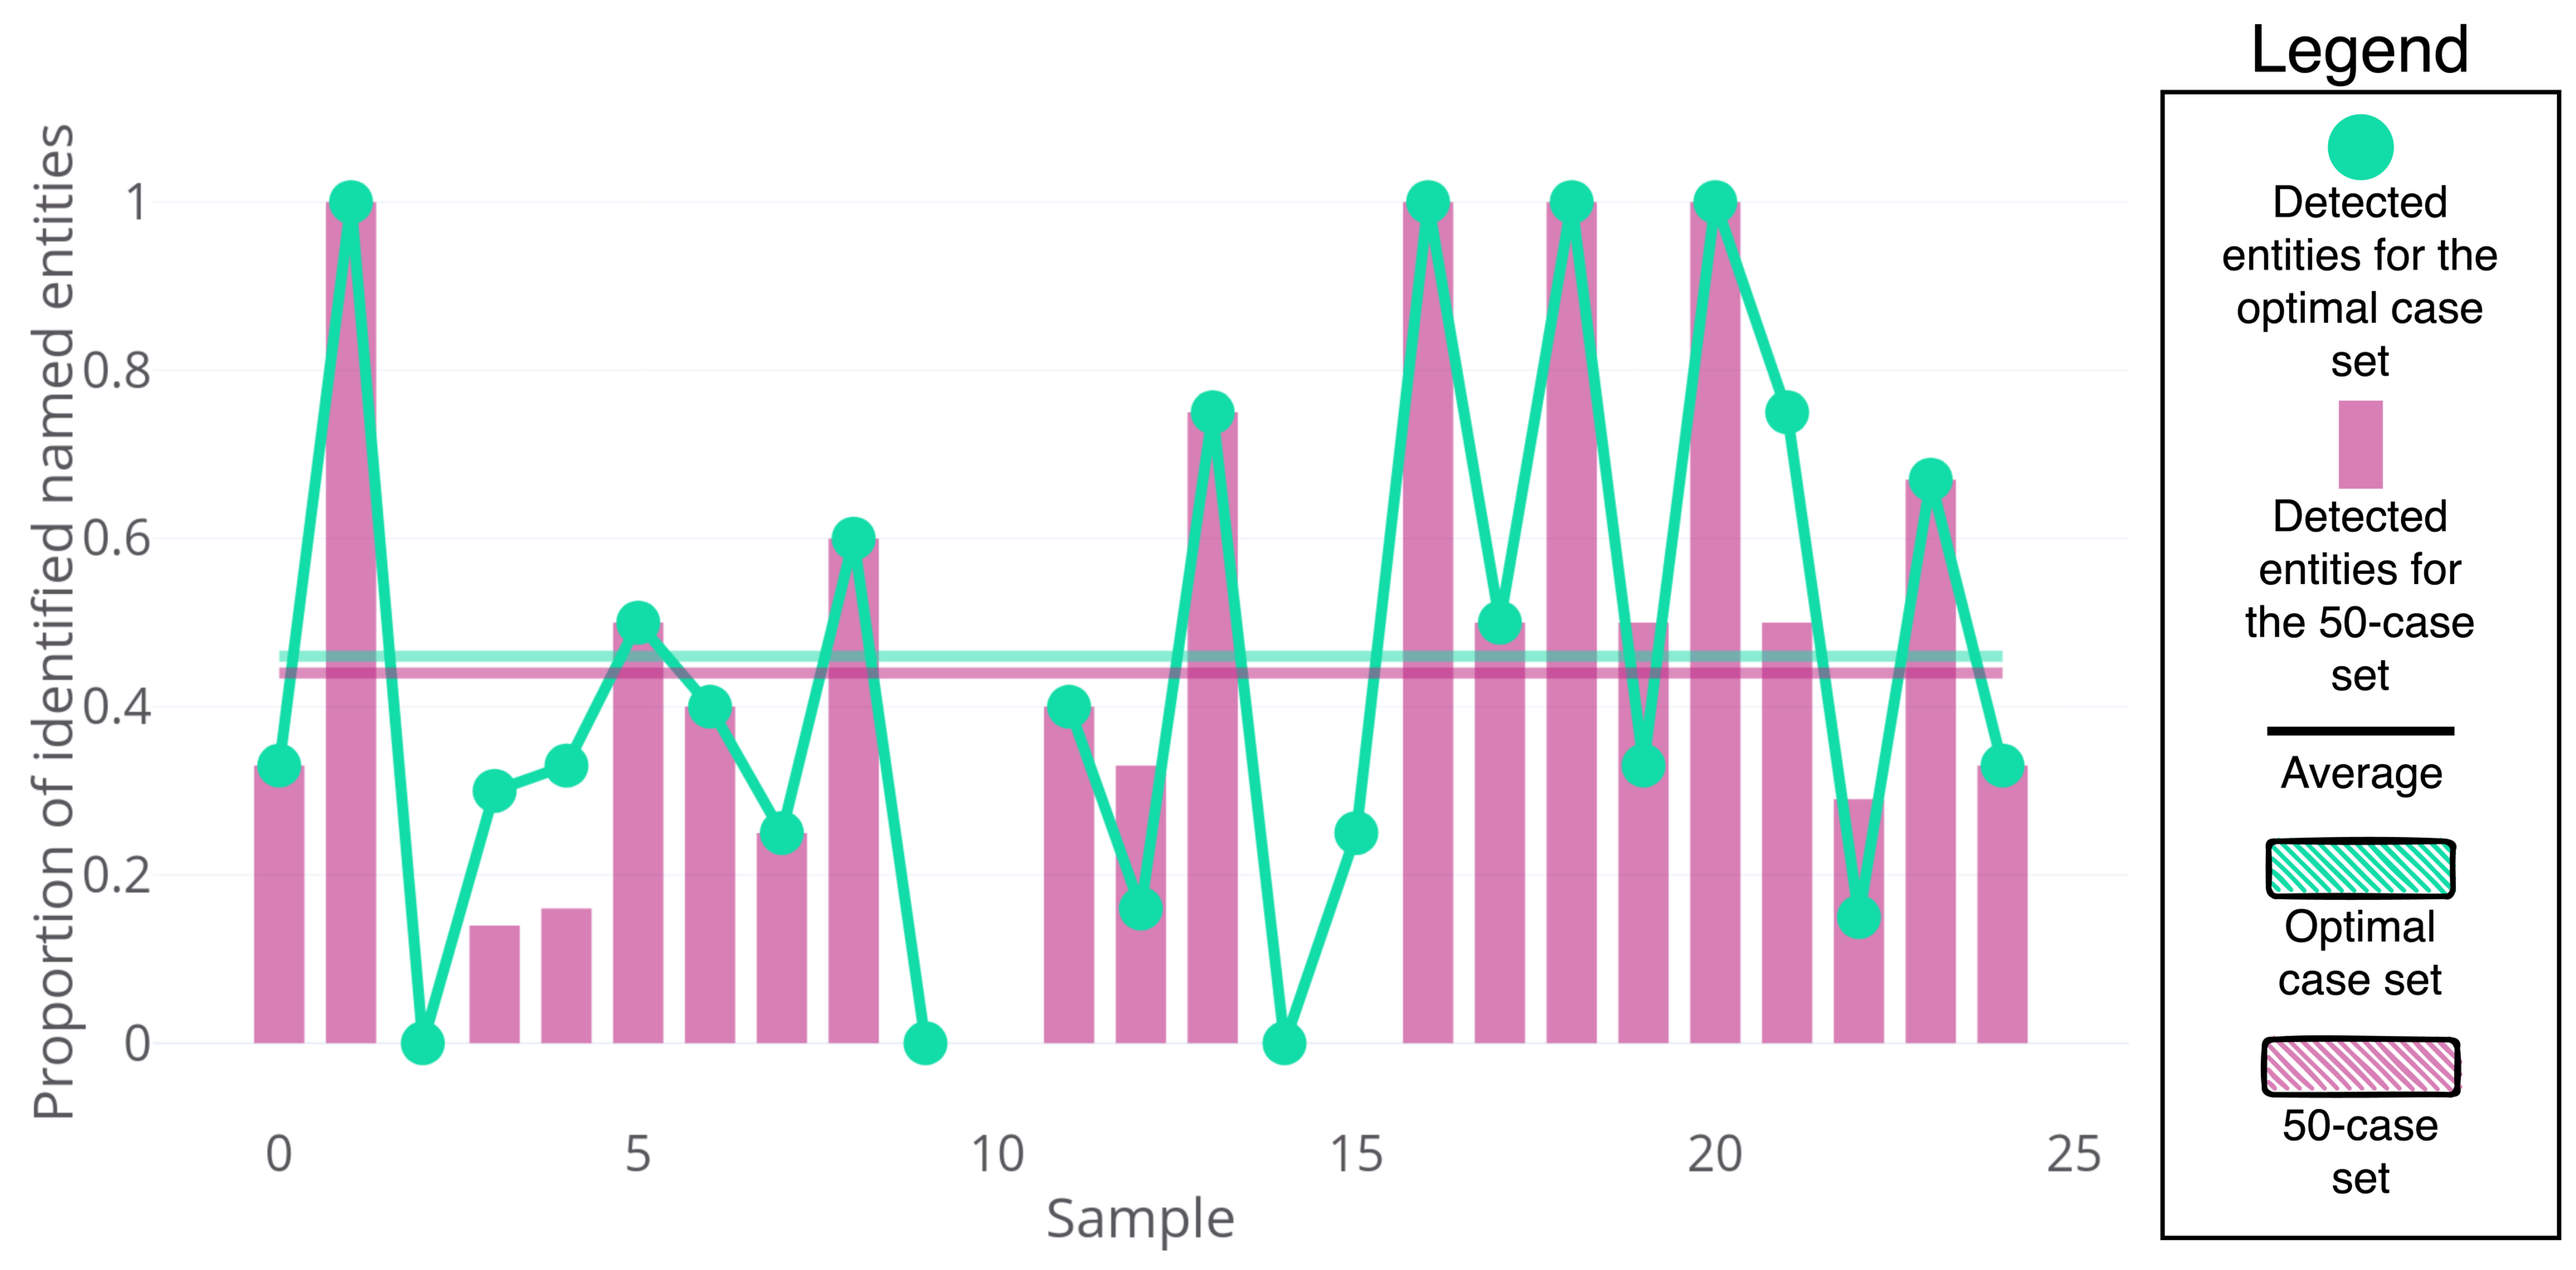
\includegraphics[width=.75\columnwidth]{5_dlintegrationkbs/figures/ecgen_entities.eps}}
    \subfigure[MIMIC-CXR  \label{fig:mimic_entities}]{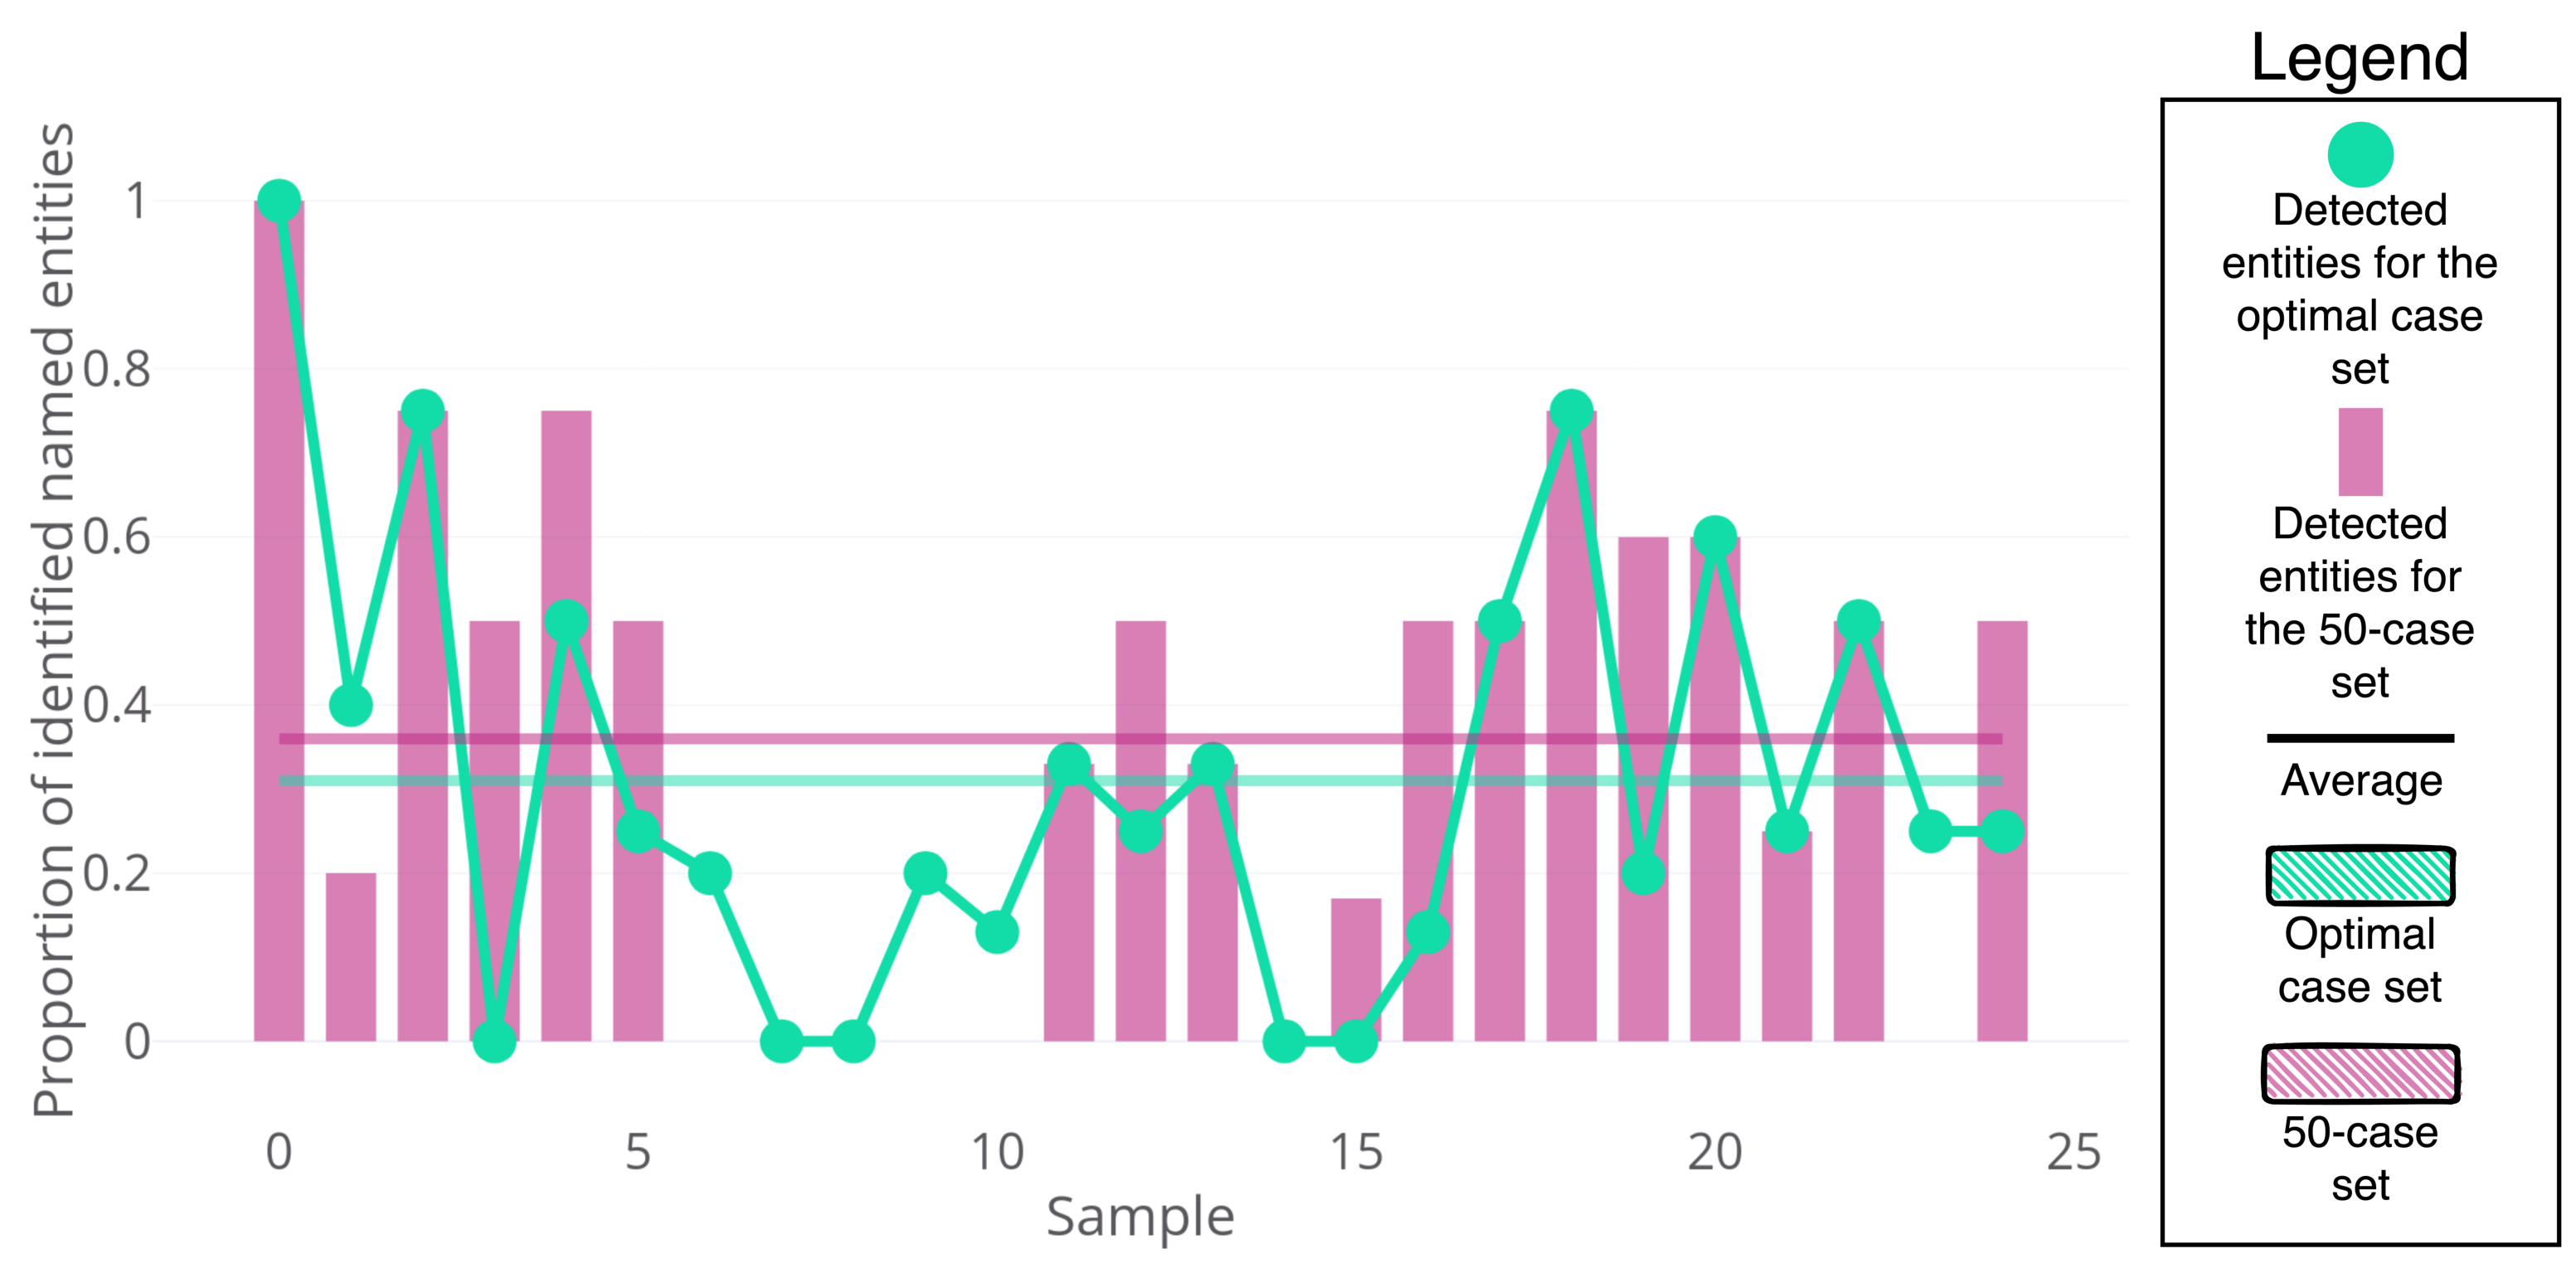
\includegraphics[width=.75\columnwidth]{5_dlintegrationkbs/figures/mimic_entities.eps}}
    \caption{Proportion of named entities correctly suggested per case on each studied dataset.}
    \label{fig:entities_comparison}
\end{figure}

Figure \ref{fig:entities_comparison} depicts the number of named entities correctly suggested by the framework. In Step 3 of the evaluation, named entities detected in the original report were replaced by escape characters as part of the corruption process. Figures \ref{fig:ecgen_entities} and \ref{fig:mimic_entities} depict the proportion of named entities stripped from the original report and correctly suggested by the system in ECGEN and MIMIC-CXR, respectively. As evidenced by the results, case base optimization induces an improvement in the number of correctly suggested entities. This phenomenon is clearly observed in ECGEN's results (Figure \ref{fig:ecgen_entities}). Only in three cases, the number of detected entities slightly decreases after case base optimization, but significantly improves in four other cases. In MIMIC-CXR (Figure \ref{fig:mimic_entities}), the result is not as consistent as in the previous dataset, which could be due to the difference in the size of the optimized case base between the two datasets. MIMIC-CXR has double the number of cases in its optimized version that ECGEN. Named entities are suggested based on the top $k$ similar cases. Hence, if the retrieved similar cases contain few named entities, it directly impacts the number of suggestions provided by the system. Increasing the value of $k$ in the retrieval could potentially correct this issue.

\color{black}
\section{Design Compliance}\label{5_sec:design_compliance}
A Case-based reasoning model comprising several boosting DL modules instantiates the insertion proposal in Section \ref{5_sec:dl_intro_kbs_methodology}. Figure \ref{fig:compliance_dl_into_kbs} denotes the specific method design parameters of the proposed framework, which are described as follows:

\begin{figure}[t]
    \centering
    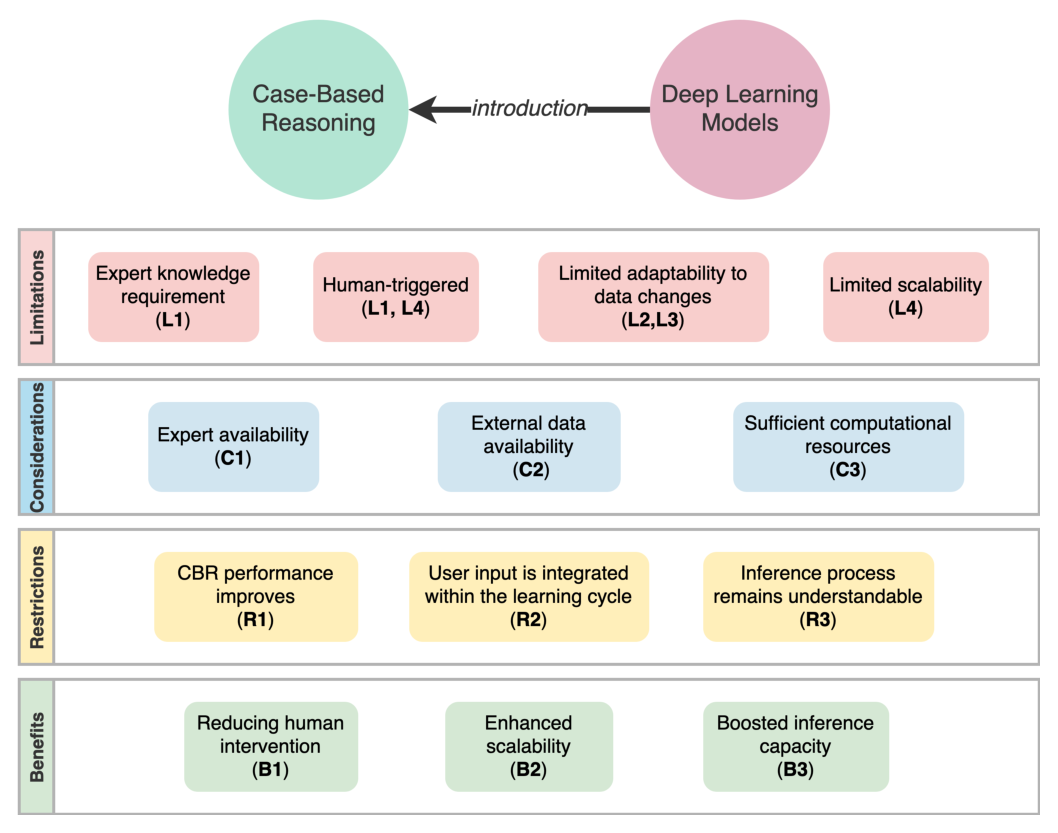
\includegraphics[width=\linewidth]{5_dlintegrationkbs/figures/Instance_DL_intro_KBS.eps}
    \caption{Overview of the design parameters of the introduction of DL models into a CBR framework. In bold, the general design parameters as depicted in \ref{fig:overview_dl_kbs_intro}.}
    \label{fig:compliance_dl_into_kbs}
\end{figure}

\subsection{Limitations}
\begin{itemize}
    \item \textbf{Expert knowledge requirement.} CBR models are highly reliant on expert input. This is particularly remarkable in the revise stage, where a panel of experts needs to manually revise the pending cases to make their inclusion in the case base effective (\ref{dl_intro_kbs_L_human}). In CBR, the system improves with the inclusion of new cases within the system. Subsequently, if no expert knowledge is available to validate the cases, the model performance remains static. 
    
    \item \textbf{Human-triggered.} In a pure CBR model, several stages are only triggered by human intervention (\ref{dl_intro_kbs_L_human}). Except in the retrieval phase, where the user can be actively involved, its influence can extend to different phases, such as revise and retain. Subsequently, the learning process may be hampered if no human intervention is available (\ref{dl_into_kbs_L_scalability}).
    
    \item \textbf{Limited adaptability to data changes.} Rule-based systems are used on a general basis in CBR models. Usually, during the reuse phase, a set of rules inferred from the existing cases is applied to devise a valid solution for the input problem. Hence, rules are only effective when the input problem resembles an existing case (\ref{dl_into_kbs_L_brittle}). The usage of rules limits the abstraction level achieved by the model to devise tailored solutions to the input problems (\ref{dl_into_kbs_L_abstraction}).
    
    \item \textbf{Limited scalability.} Reliance on expert knowledge can create a bottleneck in the system, as cases need to be manually revised before their inclusion in the case base (\ref{dl_into_kbs_L_scalability}). Similarly, in the reuse phase, the use of rule-based systems considerably limits the scalability of the system, as the rules need to be constantly updated to cover upcoming changes in the cases.
    
    
\end{itemize}
\subsection{Considerations}
\begin{itemize}
    \item \textbf{Expert availability.} In the health domain where the proposed implementation is deployed, expert knowledge is crucial for the correct behaviour of the system. Users are not required to be experts to use the system, and therefore expert knowledge must be integrated within the system so that the output is still valid. Expert knowledge must be available, at least in the initial timeline of the system, to ensure the validity of the output responses and the correct behaviour of the system (\ref{dlintrokbs_C_expert}).
    
    \item \textbf{External data availability.} DL models are data hungry, thus requiring large datasets to achieve a good performance. In the initial stages of the CBR, where the case base is not reasonably populated, the amount of available data may not be sufficient to train robust DL models. Therefore, external data may be required to train the DL model until the number of cases available is enough to replace it (\ref{dlintrokbs_C_data}).
    
    \item \textbf{Sufficient computational resources.} CBR models do not entail elevated computational power, but require sufficient storage. On the contrary, DL models may demand a higher computational power to be able to operate. Therefore, it must be ascertained that both the storage and computational resources are sufficient (\ref{dlintrokbs_C_resource}).
    
\end{itemize}
\subsection{Restrictions}
\begin{itemize}
    \item \textbf{Case-based reasoning model performance improves.} The introduction of DL models carries a computational cost. This increment in cost must be reflected in a noticeable improvement in the performance of the model to maintain a balance between benefit and cost. The proposed framework satisfices this constraint, as the inclusion of DL models induces the generation of case solutions that cannot be inferred otherwise (\ref{dlinstrokbs_R_performance}).
    
    \item \textbf{User input is integrated within the learning cycle.} CBR models are user-oriented, and therefore the validity of a given solution is not objective, but subjective to the user requirements and expectations. Subsequently, user input must play an important role in the generation of the case solution, and should be considered by the different modules to adjust their outputs accordingly. In the proposed framework, user input not only guides the retrieval process, but it is also required to correct and validate the initially proposed solution (\ref{dlintrokbs_R_user}). 
    
    \item \textbf{Inference process remains understandable.} One of the key advantages of symbolic models with respect to their subsymbolic counterparts are their transparency and interpretability. This property should be therefore preserved. In the proposed implementation, DL models are included seamlessly in the CBR cycle. Therefore, while some minor elements of the retrieve and reuse phases may be opaque, the output of each phase as a whole can be fully understood from the input (\ref{dlintrokbs_LR_interpretability}).
\end{itemize}
\subsection{Benefits}
\begin{itemize}
    \item \textbf{Reducing human intervention.} Expert knowledge is essential in the early learning stages of the CBR model to compensate the lack of cases contained in the case base. However, when the number of elements in the case base is sufficient to train robust DL models, expert knowledge may be not required as frequently. The replacement of rule-based systems by DL models reduces the need for human intervention, as DL models can automatically fit new data without external specifications (\ref{dlintrokbs_B_automatization}).
    
    \item \textbf{Enhanced scalability.} Replacing rule-based systems with DL models not only reduces the need for human intervention, but improves the scalability of the system. While rules require human intervention for validation and maintenance, thus creating potential bottlenecks, DL models operate autonomously. Therefore, reuse modules are easily and automatically kept updated with the data contained in the case base (\ref{dlintrokbs_B_scalability}).
    
    \item \textbf{Boosted inference capacity.} CBR should produce a tailored solution for a given input, which is generally obtained via rule instantiation. The solutions inferred by the rules are highly limited, as they rely on generalizations about the data, thus not capturing the particularities of each case. Moreover, they may be insufficient to deal with complex inputs where the attributes are not strictly quantitative. The inclusion of DL models not only enables the generation of solutions that could not be inferred from rules, but also enables the comparison of complex inputs, such as textual reports (\ref{dlintrokbs_B_inference}).
\end{itemize}

\section{Summary}\label{5_sec:summary}
\elvitodo{TBD cuando esté hecha la metodología para relacionar todo}